\documentclass[twoside,english]{uiofysmaster}
\usepackage[utf8]{inputenc}
\usepackage[T1]{fontenc}
\usepackage[english]{babel}
\usepackage{epsfig}
\usepackage{graphicx}
\usepackage{caption}
\usepackage{subcaption}
\usepackage{amsfonts, amssymb, amsmath}
\usepackage{listings}
\usepackage{float}
\usepackage{hyperref}
\usepackage{epstopdf}
\usepackage{nomencl}
\usepackage{tabularx}
% \usepackage{subfiles}
\usepackage{color}
\usepackage{arydshln,leftidx,mathtools}
\makenomenclature

\usepackage{pdfpages}
\usepackage[backend=bibtex]{biblatex}
% \bibliography{bibtex_ref_test.bib}
\bibliography{references.bib}

\renewcommand{\d}{\partial}
\renewcommand{\nomname}{List of Abbreviations}
% \renewcommand{\notetoself{}}{\emph{\textcolor{red}{}}}

\setlength{\headheight}{15pt}

% \usepackage{fontspec}
% \newfontfamily\listingsfont[Scale=0.85]{Droid Sans Mono}
% \lstset {
%     basicstyle=\footnotesize\listingsfont,
%     keywordstyle=\color{listingskeywordcolor}\footnotesize\listingsfont,
%     stringstyle=\color{listingsstringcolor}\footnotesize\listingsfont,
%     commentstyle=\color{listingscommentcolor}\footnotesize\listingsfont,
%     numberstyle=\gls{pde}\color{listingsnumbercolor}\footnotesize\listingsfont,
%     identifierstyle=\footnotesize\listingsfont,
% }



% compile with pdflatex --shell-escape thesis.tex
% makeindex thesis.nlo -s nomencl.ist -o thesis.nls

%opening
\author{Fredrik E Pettersen\\ f.e.pettersen@fys.uio.no}
\title{\uppercase{Multiscale modeling of diffusion processes in the brain}}
\date{June 2014}


\begin{document}

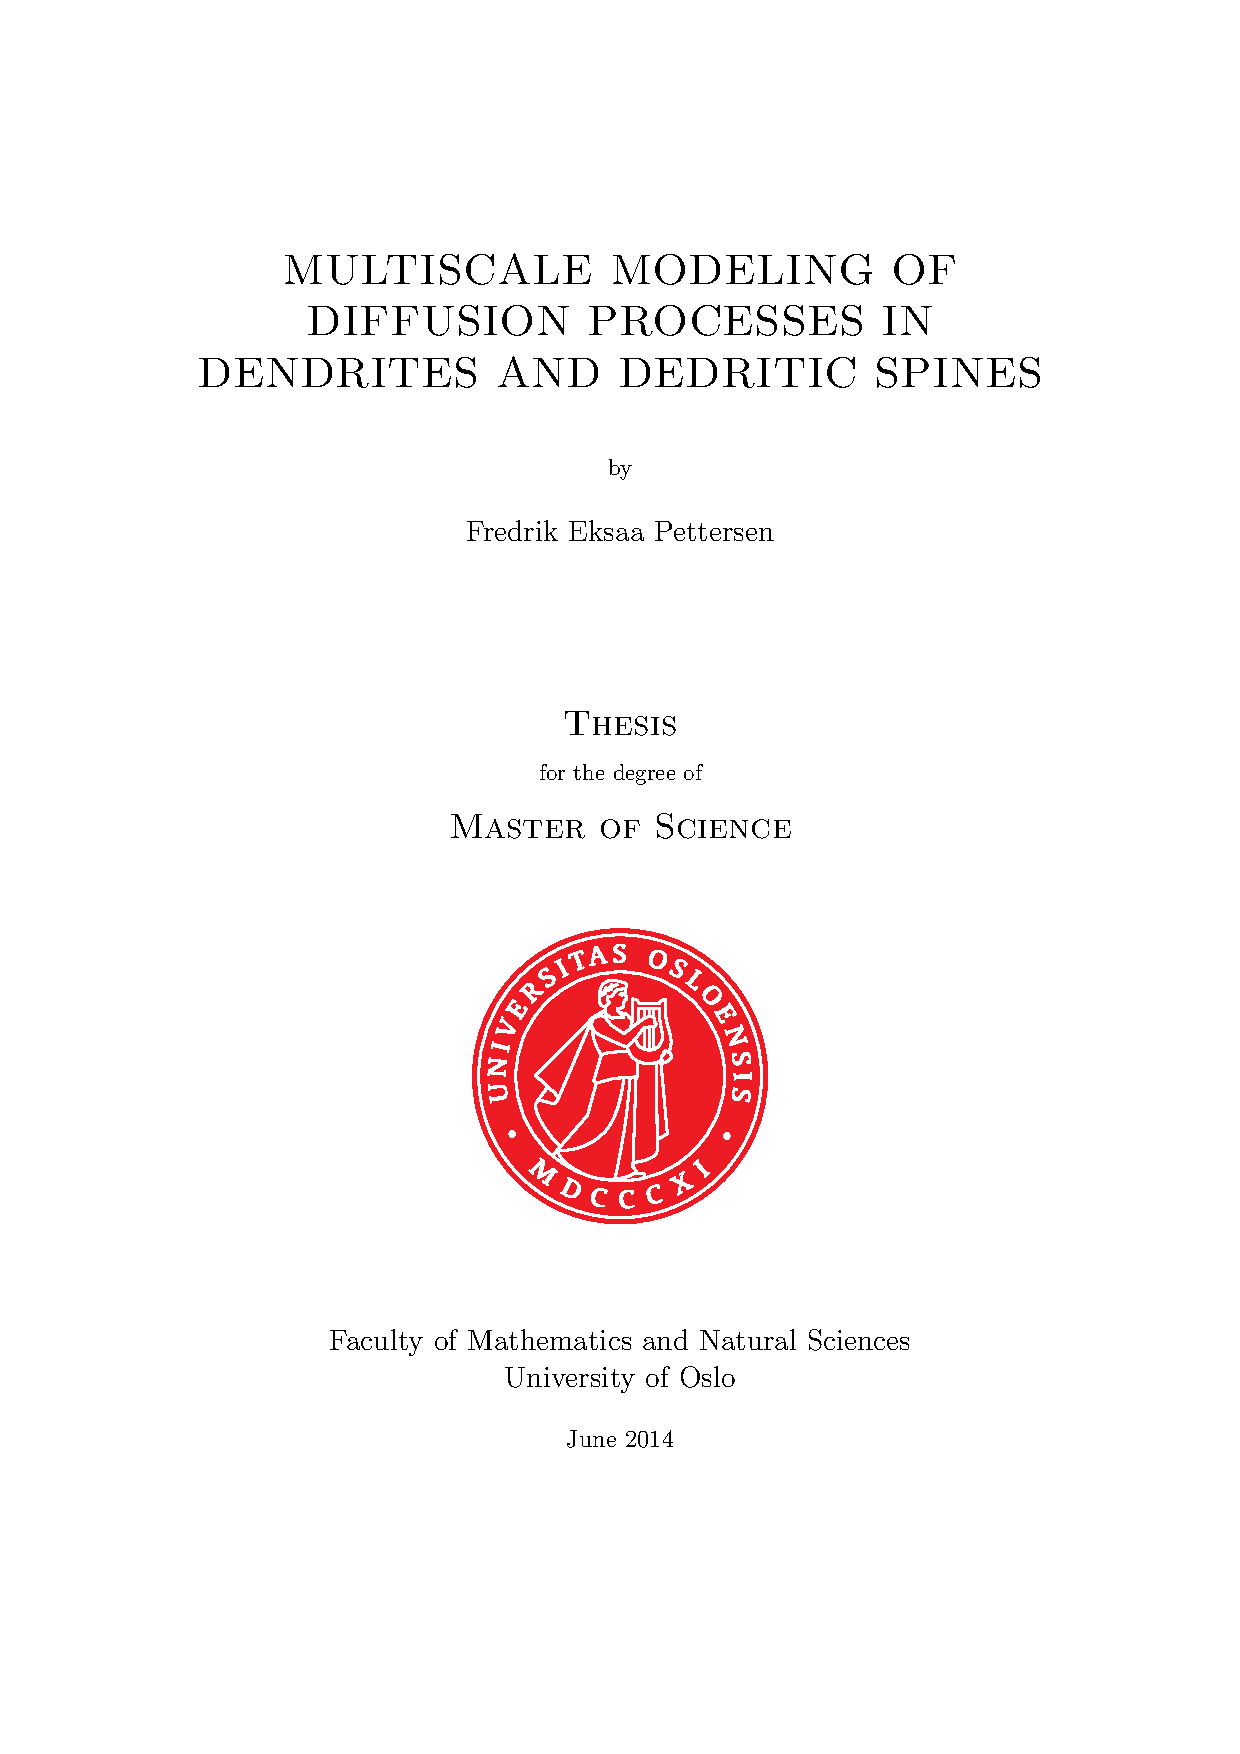
\includepdf{frontpage.pdf}
\cleardoublepage

% \begin{abstract}
% This is an abstract text.
% \end{abstract}

% \begin{dedication}
%   To someone
%   \\\vspace{12pt}
%   This is a dedication to my cat.
% \end{dedication}

% \begin{acknowledgements}
%   I acknowledge my acknowledgements.
% \end{acknowledgements}


\tableofcontents
\clearpage
\listoffigures

\clearpage
\printnomenclature

% \clearpage
% \listoftables

\chapter{Introduction}
\clearpage
Diffusion processes are extremely important in modern science, and have so many applications that it is challenging to list them all. 
Brownian motion of particles, momentum in liquids, and atomic diffusion are just some examples of processes described by the diffusion equation. \\
\noindent Both in general transport processes, and particularly in diffusion processes, there are cases in which parts of the process cannot be described by a continuum model, but the rest of the process can. 
Examples of such processes are fluid flow in nanoporous media and diffusion in the extracellular space of the brain. There are also many examples in materials design.

\noindent These types of processes can be called multi scale processes in the sense that more than one model is required to describe the entire system. Usually these are on different length scales. 
There are three obvious ways to handle multi scale problems. 
The first alternative is to ignore the problem, and assume that the chosen model can accurately solve the problem. For diffusion processes, this approach often works a lot better than it should. 
A more realistic approach is to create an intermediate scale and model. In the limit between continuum and particle dynamics this is often called a \emph{meso scale} model. 
An example of a meso scale model is dissipative particle dynamics \cite{warren1998dissipative}, where clusters of particles are modeled as individual particles. The particle clusters have different properties than the individual atoms or molecules which make up the substance. 
A final alternative is a \emph{hybrid} model.
Some hybrid models exist today, but these are mostly aimed at specific problems, like dendritc solidification \cite{plapp2000multiscale}, or hybrid fluid flow models which combine molecular dynamics and Navier-Stokes solvers \cite{o1995molecular}. 
Other hybrid solvers for diffusion processes have also been developed \cite{flekkoy2001coupling}, but they are closed in the sense that the computer code is not commonly available. \\

\noindent The aim of this masters thesis is to develop a simple, yet flexible hybrid diffusion solver from the ground and up where all parts of the theory and implementation are fully understood and transparent. 
In principle, any particle dynamics model could be used, but for the sake of verification a stochastic model has been implemented. 
This is no limitation, as the interface to the lower scale model is simple, and the lower scale model works as a standalone unit. \\

\noindent A large emphasis has been put on verification of all parts of the hybrid model. 
Both individually and for the combined, hybrid solver to verify the average behavior of the system.\\

\section{Outline}
\noindent The thesis in your hands has the following structure: \\

\noindent \emph{Chapter \ref{chapter:theory}} contains a detailed review of the coupling between the two models, as well as a look at band diagonal linear systems. \\

\noindent \emph{Chapter \ref{chapter:analysis}} defines the error estimate and shows a thorough analysis of all parts of the developed software in order to verify that it functions properly. \\

\noindent In \emph{chapter \ref{chapter:application}} the developed software is modified to describe a physical application in which a hybrid diffusion solver is demanded. \\

\noindent \emph{Chapter \ref{chapter:results}} presents and discusses the results from the verification of the computer code and the physical application. \\

\noindent Finally, \emph{chapter \ref{chapter:discussion}} discusses the thesis as a whole and looks at possible improvements and extensions that can be done. \\

\noindent The \emph{appendix} is a general guide to debugging the methods that have been implemented during this project.

\chapter{Theory}
\clearpage

This chapter will deal with random walks in general and the transition from the statistical view to PDEs. 
Different algorithms to produce random walks will be discussed, highlighting their pros and cons in light of this project along with some details which prove either problematic or helpful. 
Numerical solution of PDEs will also be discussed, also with emphasis on what is relevant for this project. 
Finally an algorithm for combining random walk diffusion solvers and normal PDE diffusion solvers will be introduced and discussed.

\section{Notation}

There will be some mathematics in this chapter, and so it might be useful to clarify on the notation used throughout the project.\\

In the following section the Gaussian distribution will be derived from the Bernoulli distribution through some expectation values such as the expected total displacement of a random walker and the expected root mean square displacement of a walker. 
Expectation values are denoted by brackets. Equation \eqref{notation:brackets} shows the expectation value of a quantity $a$. 

\begin{equation}\label{notation:brackets}
 \langle a \rangle = \sum aP(a)
\end{equation}
Note the difference between the expectation value of a quantity squared and the square of the expectation value of the same quantity, stated in equation \ref{notation:clarification}.

\begin{equation}\label{notation:clarification}
 \langle a \rangle^2 \neq \langle a^2 \rangle
\end{equation}

For the section on discretization of partial differential equations \ref{some_words_on_PDEs} some sub- and super- scripts will be used. 
To clarify; a superscript $t^n$ does not mean t to the n'th power, but $n\cdot\Delta t$ meaning the n'th time-step. 
Similarly, the subscripts denote positions on the mesh. This means, finally, that $u^n_{ij}$ denotes the numerical solution to the discretized PDE evaluated at time-step n and in the i'th point in x-direction and the j'th point in y direction:
\begin{equation*}
 u^n_{ij} = u(n\cdot\Delta t,i\cdot\Delta x, j\cdot\Delta y)
\end{equation*}

Throughout the thesis, the use of exponential functions might seem a bit inconsistent notation-wise. 
There are two different notations in use, $e^C$ and $\exp(C)$. 
The latter is mainly used when the expression $C$ is large, like a fraction, to improve readability. 
However, this is abandoned if there might be room for misconception. 
As an example, the calculations in section \ref{more_general_random_walks} are done using $e^C$ rather than $\exp(C)$ even though $C$ might be a fraction.
This is done because the exponential at some point is multiplied by a parenthesis, and where this multiplication takes place might have been unclear otherwise.

\section{Introduction to random walks}\label{introduction_to_random_walks}

The most basic random walk (\emph{is it though?}) is a walker on the x-axis which will take a step of a fixed length to the right with a probability $p$, or to the left with a probability $q=1-p$. 
Using (pseudo-) random numbers on a computer we can simulate the outcomes of a random walk. 
For each step (of which there are N) a random number, $r\in [0,1]$ is drawn from some distribution (say a uniform one) which will be the probability. 
If $r\leq p$ the walker will take a step to the left, otherwise it will take a step to the right. 
After the N steps the walker will have taken R steps to the right, and $L = N-R$ steps to the left. 
The net displacement from the origin will be $S = R-L$. \\
This simple approach is easily generalizable to two and three dimensions by having $2d$ possible outcomes from the random number, where d is the dimensionality. 
In two dimensions the walk can be split in two; first randomly choosing what dimension to perform the step in and then randomly choosing the sign of the step ($(-1)^r\cdot l$).

\subsection{Random walkers and Gaussian distribution}\label{further_introduction}
The following derivation is borrowed from a compendium in statistical mechanics by Finn Ravndal. \\
If sufficiently many walks are done, the net displacement will vary from $S=+N$ to $S=-N$ representing all steps to the right and all steps to the left respectively. 
The probability of all steps being to the right is $P_N(N) = p^N$. 
Should one of the steps be to the left, and the rest to the right the resulting net displacement will be $S = N-2$ with the probability $P_N(R = N-1) = Np^{N-1}q$. 
This can be generalized to finding the probability of a walk with a R steps to the right as 
\begin{equation}\label{bernoulli_distr}
 P_N(R) = {N\choose R}p^{R}q^{N-R}
\end{equation}
where ${N\choose R}=\frac{N!}{R!(N-R)!}$ is the number of walks which satisfy the net displacement in question, or the multiplicity of this walk in statistical mechanics terms. 
Equation \ref{bernoulli_distr} is the Bernoulli probability distribution, which is normalized.

\begin{align*}
 \sum\limits_{R=0}^N P_N(R) = (p+q)^N = 1^N = 1
\end{align*}

From this distribution important statistical properties of a walk consisting of some N steps can be calculated.
% We can use this distribution to calculate various average properties of a walk consisting of N steps. 
For example, the average number of steps to the right is

\begin{align*}
 \langle R\rangle &=  \sum\limits_{R=0}^N RP_N(R) =  \sum\limits_{R=0}^N {N\choose R}Rp^Rq^{N-R} = \\
 p\frac{d}{dp} \sum\limits_{R=0}^N {N\choose R}p^Rq^{N-R} &= p\frac{d}{dp}(p+q)^N = Np(p+q)^{N-1} = Np
\end{align*}

The average value of the net displacement is found by using $S = R-L = R-(N-R) = 2R-N$.
% From this we can also find the average value of the net displacement using $S = R-L = R-(N-R) = 2R-N$.

\begin{align*}
 \langle S\rangle = \langle2R\rangle -N = 2Np-N(p+q) = N(2p-p-q) = N(p-q)
\end{align*}
We notice that the average net displacement is greatly dependent on the relationship between $p$ and $q$, and that any symmetric walk will have an expected net displacement of zero. 
In many cases the mean square displacement is of more interest than the displacement itself, because many important large scale parameters can be related to the root-mean-square displacement. 
This can also be calculated rather straightforwardly. 
\begin{align*}
  \langle R^2\rangle =  \sum\limits_{R=0}^N R^2P_N(R) &=  \sum\limits_{R=0}^N {N\choose R}R^2p^Rq^{N-R} = \\
 \left(p\frac{d}{dp}\right)^2 \sum\limits_{R=0}^N {N\choose R}p^Rq^{N-R} &= \left(p\frac{d}{dp}\right)^2(p+q)^N \\
 = Np(p+q)^{N-1} +p^2N(N-1)(p+q)^{N-2} &= (Np)^2 +Np(1-p) = (Np)^2 +Npq
\end{align*}

Like before, the average net displacement is given as $S^2 = (2R-N)^2$ and we obtain

\begin{align*}
 \langle S^2\rangle = 4\langle R^2\rangle -4N\langle R\rangle + N^2 &= 4((Np)^2 +Npq) -4N^2p + N^2\\
 = N^2(4p^2 -4p +1) +4Npq &= N^2(2p-1)^2 +4Npq = N^2(p-q)^2 +4Npq.
\end{align*}
which for the 1D symmetric walk gives $\langle S^2\rangle =N$ and the variance, denoted $\langle\Delta S^2\rangle = \langle\langle S^2\rangle-\langle S\rangle^2\rangle$, is found by insertion as
\begin{align}
 \langle\Delta S^2\rangle &= \langle N^2(p-q)^2 +4Npq - ( N(p-q))^2\rangle= 4Npq 
\end{align}

When the number of steps gets very large the Bernoulli distribution (eq. \ref{bernoulli_distr}) can to a very good accuracy be approximated by the Gaussian distribution. 
This is most easily done in the symmetric case where $p=q=\frac{1}{2}$, but it is sufficient for the step-lengths to have a finite variance (\emph{find something to refer to}). 
The Bernoulli distribution then simplifies to
\begin{equation}
 P(S,N) = \left(\frac{1}{2}\right)^N\frac{N!}{R!L!}
\end{equation}
on which we apply Stirling's famous formula for large factorials $n!\simeq\sqrt{2\pi n}\cdot n^ne^{-n}$.
\begin{align*}
 P(S,N) &= \left(\frac{1}{2}\right)^N\frac{N!}{R!L!} \\
 &= \exp\left(-N\ln2+\ln\sqrt{2\pi N}+N\ln N - \ln\sqrt{2\pi R} -R\ln R - \ln\sqrt{2\pi L} - L\ln L \right) \\
 &= \sqrt{\frac{N}{2\pi RL}}\exp\left(-R\ln\frac{2R}{N}-L\ln\frac{2L}{N}\right)
\end{align*}

Where we have used $R+L=N$. 
Inserting $\frac{2R}{N}=1+\frac{S}{N}$ and $\frac{2L}{N}=1-\frac{S}{N}$ and expanding the logarithms to first order results in
\begin{align*}
 P(S,N) &= \sqrt{\frac{N}{2\pi RL}}\exp\left(-\frac{N+S}{2}\frac{S}{N} + \frac{N-S}{2}\frac{S}{N}\right)\\
 &= \sqrt{\frac{N}{2\pi RL}}\exp\left(-\frac{S^2}{2N}\right)
\end{align*}

Then inserting $RL=\frac{N^2-S^2}{4}$ in the prefactor, and approximating $1-\frac{S^2}{N^2}\simeq1$ results in a discrete Gaussian distribution (eq. \ref{descrete_gaussian_distr}) with $\langle S\rangle = 0$  and $\langle S^2\rangle = N$.

\begin{equation}\label{descrete_gaussian_distr}
 P(S,N) =\sqrt{\frac{2}{\pi N}}\exp\left(\frac{-S^2}{2N}\right)
\end{equation}

A continuous final position can be derived by assuming that the walker is moving on the x-axis, and letting the step-length, a, get small. 
The final position is now the continuous variable $x=Sa$.
% If we keep assuming that the walker is on the x-axis, and let the step length, a, get small the final position will be $x=Sa$ which we can assume is a continuous variable. 
Similarly the time interval between each step, $\tau$ is assumed to be small, and the walker now runs for a continuous time-variable $t=N\tau$.
% Similarly, we let the time interval between each step, $\tau$, be small and let the walk run for a continuous time $t=N\tau$. 
This changes the distribution \ref{descrete_gaussian_distr} to
\begin{equation}
 P(x,t) = \frac{1}{2a}\sqrt{\frac{2\tau}{\pi t}}\exp\left(-\frac{x^2\tau}{2a^2t}\right). 
\end{equation}
The prefactor $\frac{1}{2a}$ is needed to normalize the continuous probability distribution since the separation between each possible final position in walks with the same number of steps is $\Delta x=2a$. 
Introducing the diffusion constant
\begin{equation}
D = \frac{a^2}{2\tau} 
\end{equation}
makes the distribution
\begin{equation}
 P(x,t) = \sqrt{\frac{1}{4\pi Dt}}\exp\left(-\frac{x^2}{4Dt}\right)
\end{equation}

Introducing $x$ also gives us the expectation value and variance of x on a form which will be useful later. 

We have $x=Sa$ which means 
$$\langle x\rangle=a\langle S\rangle$$ 
and 
$$\langle x^2\rangle=a^2\langle S^2\rangle$$
Finally, the variance is found by insertion $\langle \Delta x^2\rangle$
\begin{equation}\label{random_walk_variance}
 \langle \Delta x^2\rangle = \langle\langle x^2\rangle -\langle x\rangle^2\rangle = \langle a^2\langle S^2\rangle -a^2\langle S\rangle^2\rangle = 4Npqa^2
\end{equation}


\subsection{More general Random Walks}\label{more_general_random_walks}

In the more general case, the position of a random walker, $\vec{r}$ at a time $t_i$ is given by the sum
\begin{equation}\label{brownian_motion}
 \vec{r}(t_i)=\sum\limits_{j=0}^i \Delta \vec{x}(t_j)
\end{equation}
where $\Delta \vec{x}(t_j) = \left(\Delta x(t_j),\Delta y(t_j),\Delta z(t_j)\right)$ in 3D. Each $\Delta x,\Delta y,\Delta z$ is a random number drawn from a distribution with a finite variance $\sigma^2 = \langle\Delta x^2\rangle$. 
By the central limit theorem, any stochastic process with a well defined mean and variance can, given enough samples, be approximated by a Gaussian distribution. 
This means that the probability of finding the walker at some position x after M steps is 
\begin{equation}
 P(x,M)\propto e^{-\frac{x^2}{2M\sigma^2}}
\end{equation}
Recall that the actual Gaussian distribution is 
$$
\frac{1}{\sqrt{2\pi\sigma^2}}\exp\left(\frac{(n-\mu)^2}{2\sigma^2}\right)
$$

Introducing an Einstein relation $\sigma^2 = 2dD\Delta t$ and the obvious relation $t = M\Delta t$ results in a more desirable exponent. 

\emph{The introduction of the Einstein relation might put some restrictions on the model.}
Normalizing the expression gives
\begin{equation}\label{rw_gaussian_distribution}
 P(x,t) = \sqrt{\frac{1}{4Dt}}\exp\left(-\frac{x^2}{4Dt}\right)
\end{equation}

A large number, N, of walkers can be described by their concentration $C(x,t) = NP(x,t)$.
% If we have a large number, N, of walkers, their concentration will be $C(x,t) = NP(x,t)$. 
The concentration is conserved, so any amount that flows out of an area must reflect as a decrease in concentration. 
This is expressed by the flow of concentration
\begin{equation}
 \frac{\d C}{\d t} -\nabla\cdot\vec{J} = S
\end{equation}
where $\vec{J}$ is the flow vector and S is a source term which for now is zero.
Through Fick's first law the diffusive flux is related to the concentration gradient $\vec{J} = -D\nabla C$. 
Inserting this gives
\begin{equation}\label{simple_diffusion_equation}
 \frac{\d C}{\d t} = \nabla\cdot \left(D\cdot\nabla C\right)
\end{equation}
which is the diffusion equation.
Insertion of the Gaussian distribution \eqref{rw_gaussian_distribution}) verifies that the Gaussian distribution fulfills the diffusion equation. 
Starting with only the time derivative gives
\begin{align*}
 \frac{\d P}{\d t} &= -\frac{4\pi De^{-\frac{x^2}{4Dt}}}{2\sqrt{(4\pi Dt)^3}}+\frac{x^2e^{-\frac{x^2}{4Dt}}}{4Dt^2\sqrt{4\pi Dt}} \\
 &= e^{-\frac{x^2}{4Dt}}\left(\frac{8Dx^2}{2\sqrt{\pi}(4Dt)^{5/2}} -\frac{(4D)^2t}{2\sqrt{\pi}(4Dt)^{5/2}}\right)\\
 &= \frac{4De^{-\frac{x^2}{4Dt}}(x^2-2Dt)}{\sqrt{\pi}(4Dt)^{5/2}}
\end{align*}
 Which is balanced by the spatial derivative
\begin{align*}
 D\frac{\d^2 P}{\d x^2} &= \frac{D}{\sqrt{4\pi Dt}}\frac{\d}{\d x}\left[-e^{\frac{-x^2}{4Dt}}\left(\frac{-2x}{4Dt}\right)\right]\\
 &= \frac{2D}{4Dt\sqrt{4\pi Dt}}e^{\frac{-x^2}{4Dt}}\left[1-x\left(\frac{2x}{4Dt}\right)\right] \\
 &= \frac{4De^{-\frac{x^2}{4Dt}}(x^2-2Dt)}{\sqrt{\pi}(4Dt)^{5/2}}
\end{align*}
meaning that the diffusion equation is satisfied.

\subsection{Choosing random walk algorithm}\label{choosing_random_walk_algorithm}

The simplest random walk model, which places walkers on discrete mesh points and uses a fixed step length, has been used with great success to model diffusion processes. 
Farnell and Gibson discuss this in their article \cite{farnell2005monte}. 
In this project we will be torn between choosing a realistic algorithm to advance the random walkers, like Brownian motion or to go for simplicity. 
That being said, by the central limit theorem both models will after some time-steps be described by a Gaussian distribution meaning that on the PDE scale we will not know the difference. 
Hence it will make no sense to not use the simplest random walk model.
Note that it will be quite easy to change the algorithm used for random walks, and so we have not locked ourselves to anything yet.

\subsection{Random walks and anisotropy}\label{random_walks_and_anisotropy}

Although the self diffusion problem, which is what we are looking at with diffusing particles in and out of dendritic spines is not anisotropic on its own, there might be some possible applications which require describing anisotropic diffusion of random walkers.
There is reason to believe that an anisotropic diffusion process on the PDE level will lead to an anisotropic random walk model as well, but how should this be modeled. 
Simply replacing the diffusion constant by a function $D = D(\vec{x})$ (see eq \eqref{steplength}) is a natural first approximation, but this will not quite be sufficient as Farnell and Gibson point out \cite{farnell2005monte}. 
Through their experiments they found that only adjusting the step-length will not improve the error noticeably and reasoned that this is because the walkers are still as likely to jump in both directions (right or left in 1d), and that the stepsize is the same in both cases, hence the model does not resemble anisotropy. 
They went on to introduce an adjusted step-length and an adjusted step probability, a solution they landed on after trial and error. 
The expressions they proposed are listed in equations \eqref{farnell_and_gibson_1} to \eqref{farnell_and_gibson_5}. 

\begin{equation}\label{farnell_and_gibson_1}
 \Delta_p(x) = \frac{1}{2}\left(L(x) + L(x +\Delta_p(x))\right) \to L(x) +\frac{1}{2}L(x)L'(x)
\end{equation}
\begin{equation}\label{farnell_and_gibson_2}
 \Delta_m(x) = \frac{1}{2}\left(L(x) + L(x -\Delta_m(x))\right) \to L(x) +\frac{1}{2}L(x)L'(x)
\end{equation}

where $L(x)$ is defined in equation \ref{farnell_and_gibson_3} and $\Delta_p(x)$ and $\Delta_m(x)$ are the adjusted step-lengths to the right and left, respectively.

\begin{equation}\label{farnell_and_gibson_3}
L(x) = \sqrt{2D(x)\Delta t}
\end{equation}
The adjusted jump probabilities $T_r(x)$ and $T_l(x)$ which are the probabilities for a walker at position x to jump right or left, respectively are defined in equations \eqref{farnell_and_gibson_4} and \eqref{farnell_and_gibson_5}

\begin{equation}\label{farnell_and_gibson_4}
T_r(x) = \frac{1}{2} +\frac{1}{4}L'(x)
\end{equation}
\begin{equation}\label{farnell_and_gibson_5}
T_l(x) = \frac{1}{2} -\frac{1}{4}L'(x)
\end{equation}
Notice that the adjusted step-length first proposed is still a part of the final expressions.


\subsection{Random walks and drift}\label{random_walks_and_drift}

Another point which should be addressed is diffusion with a drift term, $\frac{\d u}{\d x}$. 
% Another point we have yet to say something about is diffusion that has a drift term, $\frac{\d u}{\d x}$. 

Initially one thought that diffusion in the ECS of the brain was governed by a drift term, but the modern perception is that this drift term is in the very least negligible \cite{nicholson2001diffusion}. 
Though it is unlikely that we will include a drift term in our model, we will say a few words about it here since it is of importance in other applications and might be a natural extension at some point, should someone else use this work.\\
We model random walkers with drift by simply adding some vector to the Brownian motion model, thus forcing all walkers to have a tendency to walk a certain direction. 
This approach can also be used in the fixed steplength (or variable steplength in the anisotropic case)  if we express the new step, $\vec{s}$, as
\begin{align*}
 \vec{s} = (\pm l \text{ or }0,\pm l \text{ or }0) +\vec{d}
\end{align*}
where $\vec{d}$ denotes the drift of the walker.\\
We can set up the continuity equation for a concentration, $C(x,t) = NP(x,t)$ of random walkers which are affected by a drift.
\begin{equation}
 \frac{\d C}{\d t} +\nabla\cdot\vec{j} = S
\end{equation}
Where $\vec{j}$ denotes the total flux of walkers through some enclosed volume and $S$ is a source/sink term. 
Since the walkers are affected by drift the flux will consist of two terms; $\vec{j} = \vec{j}_{diff}+\vec{j}_{drift}$. 
From Fick's first law we know that $\vec{j}_{diff} = -D\nabla C$. 
The second flux term is the advective flux which will be equal to the average velocity of the system; $\vec{j}_{drift} = \vec{v}C$. 
Inserting this in the continuity equation gives us the well known convection diffusion equation \eqref{convection_diffusion_equation}.
\begin{equation}\label{convection_diffusion_equation}
 \frac{\d C}{\d t} = \nabla\cdot\left(D\nabla C\right)-\nabla\cdot\left(\vec{v}C\right) + S
\end{equation}
Which in many cases will simplify to
\begin{equation}
 \frac{\d C}{\d t} = D\nabla^2 C-\vec{v}\cdot\nabla C
\end{equation}

In order to determine all the parameters of the convection diffusion equation \eqref{convection_diffusion_equation} we will need to go through some of the calculations from section \ref{introduction_to_random_walks}. 
The situation is the same, a walker in one dimension which can jump left or right, but this time will also move a finite distance $d$ each time-step. 
This will make the expected net displacement
\begin{equation*}
 \langle S\rangle = R-L +Nd = N(p-q) + Nd
\end{equation*}
and the expected mean square displacement
\begin{equation*}
 \langle S^2\rangle = (2\langle R\rangle -N)^2 +(Nd)^2 = N^2(p-q)^2 +4Npq +(Nd)^2
\end{equation*}
which in turn gives us the variance
\begin{align*}
 \langle \Delta S^2\rangle &= \langle\langle S^2\rangle-\langle S\rangle^2\rangle \\
 &= N^2(p-q)^2 +4Npq +(Nd)^2 - N^2(p-q)^2 -(Nd)^2 \\
\langle \Delta S^2\rangle &= 4Npq
\end{align*}
This shows us that the variance is untouched by the drift term, but not the mean which for the symmetric case is $\langle S\rangle = Nd$. 
When we convert this to the continuous variables $x$ and $t$ we get the solution shown in equation \ref{solution_convection_diffusion_eq}.
\begin{equation}\label{solution_convection_diffusion_eq}
 C(x,t) = \frac{N}{\sqrt{4\pi Dt}}\exp\left(-\frac{(x-vt)^2}{4Dt}\right)
\end{equation}
Where $v = \frac{d}{\Delta t}$ is the velocity of the concentration and $D$ is the well known diffusion constant, inserted from the Einstein relation $\sigma^2 = 2D\Delta t$.\\

%%%%%% Not sure if this should be included %%%%%%%%%

% The only problem with the solution \ref{solution_convection_diffusion_eq} is that it is invalid for $t=0$. 
% In order to use it we will need an initial condition which fits the rest of the solution. 
% We try and find this by first checking by simulation if it converges towards some initial solution as $t\to0$ and if so, extrapolate this to $t=0$ as the initial condition. 
% Figure \ref{convection_diffusion_eq_initial_condition} shows the result of this little experiment, and as we clearly see it does diverge as $t\to0$. 
% However, it also converges to a Dirac delta function, $\delta(x)$ which is defined by its properties
% \begin{align*}
% \delta(x) = \begin{cases} +\infty, & x = 0 \\ 0, & x \ne 0 \end{cases}
% \end{align*}
% and
% \begin{equation*}
%  \int_{-\infty}^\infty \delta(x) \, dx = 1
% \end{equation*}
% The Dirac delta function often sought as an initial condition in experimental setups for measurements on diffusion processes because of its compatibility with a variety of diffusion equations, and should do a very good job in our numerical setup as well. 
% 
% \begin{figure}[H]
%  \centering
%  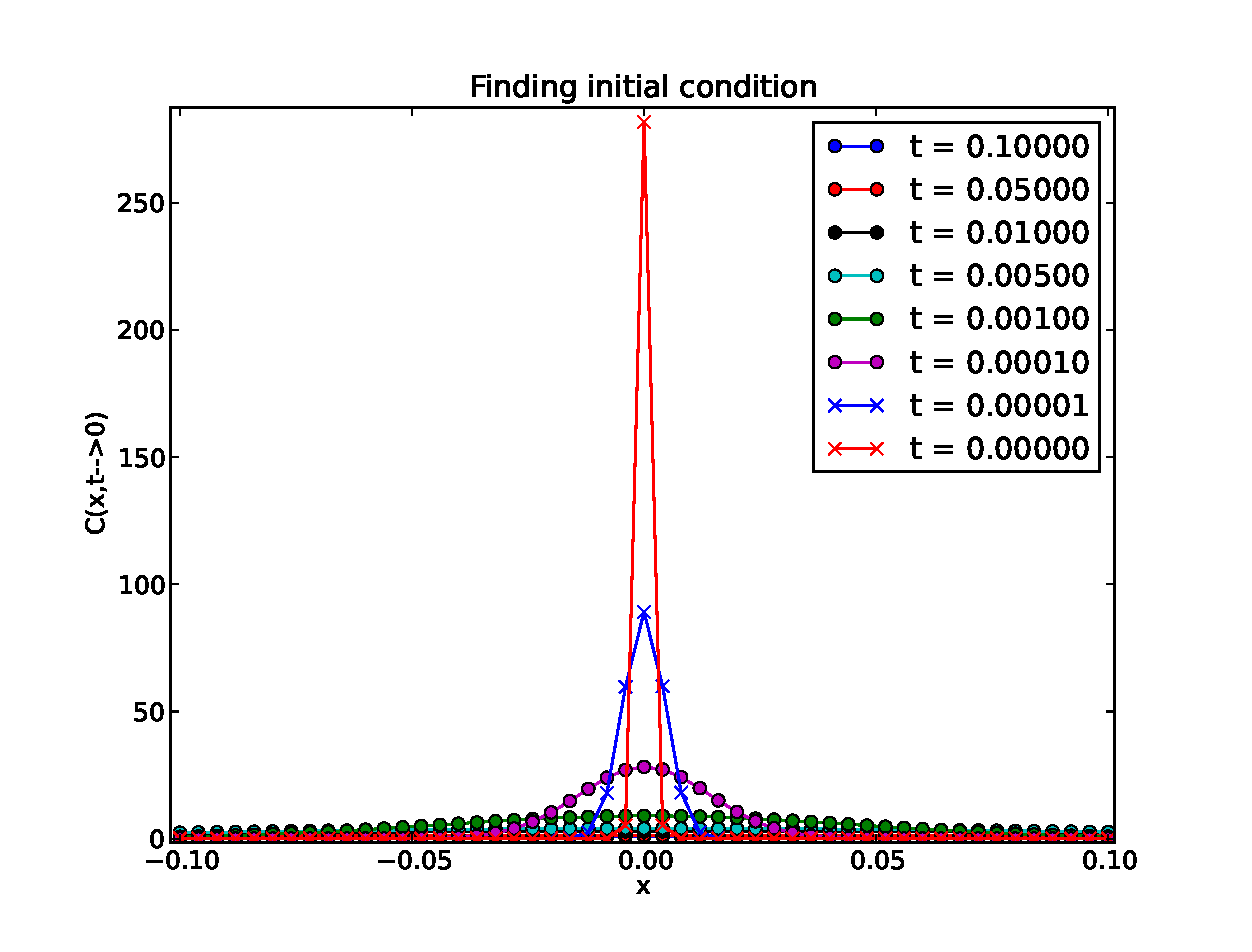
\includegraphics[scale=0.7]{Figures/convection_diffusion_eq_initial_condition.eps}
%  \caption[Initial condition for convection diffusion]{Experiment to determine the initial condition of equation \ref{solution_convection_diffusion_eq}}
%  \label{convection_diffusion_eq_initial_condition}
% \end{figure}

\subsection{Pseudo-random numbers}

This is also a large mathematical field which will only be touched in this thesis. 
Further reading can be found in \emph{Some RNG thing. Preferably be Gerorge Marsagla}. 

Although modern technology has made true randomness available, we do not currently have access to this and are limited to pseudo-random numbers. 
For all purposes in this thesis, pseudo-randomness is presumed adequate. 

A pseudo random number generator (RNG\nomenclature{RNG}{(pseudo) random number generator}) is essentially a function which produces seemingly random numbers through a series of operations. 
These operations often rely on other, engineered numbers which will maximize the RNGs period. 
A period is the number of function calls which can be performed before the RNG starts producing the same sequence of numbers. 
Naturally this period should be as large as possible. 
There are quite a lot of methods to produce pseudo-random numbers \emph{cite a review article or something}, but only two are implemented in this project (not counting the built in RNGs in the ``cmath'' and ``armadillo'' modules). 

\subsubsection{ran0}

This is a simple RNG borrowed from \cite{hjorth2011computational}. 
It is very fast, and simple to implement and use given that you know the engineered unlikely numbers it uses. 
The period of ran0 on the other hand is rather small, only $\sim 10^8$. For short simulations this will not be a problem, however.

\subsubsection{Five seeded xor-shift}

This is a more complicated algorithm developed by George Marsagla. 
It uses five seeds which are all updated every time it is called to make a pseudo-random 64-bit unsigned integer (\emph{check this}), which can be converted to a double. 
Implementing this algorithm is intricate, but it is found written out on the internet (\emph{Be very careful about this, and cite something}). 
As opposed to the ran0 algorithm this uses a series of bitshifts to produce the random numbers and update the seeds. 
It is not as fast as ran0, but only some $10-30\%$ slower. 
Because of the five seeds used, however, this algorithm has a period of $\sim10^{48}$ (\emph{This needs to come from somewhere}) making it more than good enough for most MC-simulations I have heard about, and certainly for this project.

\section{Some words about partial differential equations}\label{some_words_on_PDEs}

\subsection{Finite Difference Methods}\label{finite_difference_methods}

Although there are a few methods for solving PDEs numerically, this project will focus on finite difference methods (FDM)\nomenclature{FDM}{Finite Difference Methods}. 
This is done both for simplicity and because, as will be argued later, there is no need for very accurate solvers due to the error terms arising from random walk solvers. 

Solution of PDEs through FDMs is done by approximating a continuous axis by a discontinuous mesh, and likewise the continuous PDE is approximated by its value at the discontinuous mesh-points. 
The derivatives in the PDE are then approximated by finite differences through the definition of the derivative \eqref{derivative_definition}, replacing the limit of $h$ with the  finite discretization parameter $h$.

\begin{equation}\label{derivative_definition}
 f\!\,'(x) = \lim_{h\to 0} \frac{f(x +h) - f(x)}{h},
\end{equation}

The terms explicit and implicit scheme will also be used. 
An explicit scheme is a numerical scheme which solves a PDE numerically by using values which have already been calculated. 
A typical example of this would be to evaluate the spatial derivative at the previous time-step seeing as this has been calculated already. 
Implicit schemes typically tries to use values which have yet to be calculated in order to calculate new values. 
This can for example be achieved by evaluating the spatial derivative at the time-step which is being calculated, leading to a system of linear equations (see section \ref{discretizing} to see how this is done).

Numerical solution of PDEs is an enormous and important field, which cannot be done justice by a presentation here. 
For more on numerical solution of PDEs in general, consult \cite{} or \cite{}.

\subsection{Discretizing}\label{discretizing}

To maintain a bit of generality, the (potentially) anisotropic diffusion equation in 2d will be discretized. 
The extension to 3d is trivial, as is the 1d version. 
The drift term will be omitted in the beginning because this also results in a simple addition to the numerical scheme. The equation to be discussed is 

\begin{equation}
 \frac{\d u}{\d t} = \nabla(D\cdot\nabla u) +f
\end{equation}

where f is some source term. 
The final expression and scheme will depend on how the time derivative is approximated, but the spatial derivative will have the same approximation. \\
The innermost derivative is done first in one dimension, generalization to more dimensions is trivial, and will consist of adding the same terms for the y and z derivatives. 

\begin{align*}
 \left[\frac{d}{dx}u\right]^n \approx \frac{u^n_{i+1/2}-u^n_{i-1/2}}{\Delta x}
\end{align*}

Where the derivative is approximated around the point $x_i$. 
Inserting $\phi(x)=D\frac{du}{dx}$ simplifies the outermost derivative, which will also be done in one dimension.

\begin{align*}
  \left[\frac{d}{dx}\phi\right]^n \approx \frac{\phi^n_{i+1/2}-\phi^n_{i-1/2}}{\Delta x}
\end{align*}

Inserting for $\phi$ gives the important intermediate step

\begin{align*}
 \frac{\phi^n_{i+1/2}-\phi^n_{i-1/2}}{\Delta x} = \frac{1}{\Delta x^2}\left(D_{i+1/2}(u^n_{i+1}-u^n_{i+1}) -D_{i-1/2}(u^n_{i}-u^n_{i-1})\right)
\end{align*}

Since the diffusion constant can only be evaluated at the mesh points (or strictly speaking since it is a lot simpler to do so), an approximation $D_{i\pm1/2}\approx0.5(D_{i\pm1}+D_i)$ is used. 
Inserting this results in

\begin{align*}
 \nabla D\nabla u\approx\frac{1}{2\Delta x^2}\left((D_{i+1,j}+D_{i,j})(u_{i+1,j}-u_{i,j})-(D_{i,j}+D_{i-1,j})(u_{i,j}-u_{i-1,j})\right) \\
 +\frac{1}{2\Delta y^2}\left((D_{i,j+1}+D_{i,j})(u_{i,j+1}-u_{i,j})-(D_{i,j}+D_{i,j-1})(u_{i,j}-u_{i,j-1})\right)
\end{align*}

The discretization of the time-derivative is where a difference between the two schemes used in this project can be seen. 
When ordinary differential equations are discretized one can clearly see how this difference arises, and so the PDE \nomenclature{PDE}{Parital Differential Equation} is written in a new notation using some general operation, $P$ like the double spatial derivative

\begin{equation}
 D_t u = Pu
\end{equation}

Introducing the general discretization of the time derivative gives equation \eqref{theta_rule} known as theta-rule. 
Setting $\theta = 0$ yields the Forward Euler (FE\nomenclature{FE}{Forward Euler}) discretization, and $\theta = 1$ the Backward Euler (BE\nomenclature{BE}{Backward Euler}) discretization. 

\begin{equation}\label{theta_rule}
 \frac{u^{n+1}-u^n}{\Delta t} = P\left(\theta u^{n+1} +(1-\theta)u^n\right)
\end{equation}

From the theta rule it is clear that the only difference between the FE and BE scheme is at what time-step the right-hand-side of the equation is evaluated. 
The theta-rule can give other schemes as well, using some weighted average of the right-hand-side at $t^n$ and $t^{n+1}$ but these are considered irrelevant in this project. 
Equation \ref{FE_scheme_1D} summarizes what has been done so far by writing out the FE discretization the way it will be implemented in 1d.

\begin{align}\label{FE_scheme_1D}
 u^{n+1}_i = \frac{\Delta t}{2\Delta x^2}\left((D_{i+1}+D_{i})(u^n_{i+1}-u^n_{i})-(D_{i}+D_{i-1})(u^n_{i}-u^n_{i-1})\right) + u^n_i
\end{align}

We will come back to the FE discretization when we discuss stability later. \\
% Looking at the BE discretization which is written out in 1d in equation \ref{BE_scheme_1D} we notice that there are quite a few more unknowns per mesh-point. 
The BE discretization has more unknowns to be found at each mesh-point, as equation \ref{BE_scheme_1D} shows.

\begin{align}\label{BE_scheme_1D}
 u^{n+1}_i = \frac{\Delta t}{2\Delta x^2}\left((D_{i+1}+D_{i})(u^{n+1}_{i+1}-u^{n+1}_{i})-(D_{i}+D_{i-1})(u^{n+1}_{i}-u^{n+1}_{i-1})\right) + u^n_i
\end{align}

Writing out the calculations for a small mesh reveals a pattern which can be exploited.
\begin{align*}
 &u^{n+1}_0 =  \frac{\Delta t}{2\Delta x^2}\left(2(D_{0}+D_{1})(u^{n+1}_{1}-u^{n+1}_{0})\right) + u^n_0\\
 &u^{n+1}_1 = \frac{\Delta t}{2\Delta x^2}\left((D_{2}+D_{1})(u^{n+1}_{2}-u^{n+1}_{1})-(D_{1}+D_{0})(u^{n+1}_{1}-u^{n+1}_{0})\right) + u^n_1\\
 &u^{n+1}_2 = \frac{\Delta t}{2\Delta x^2}\left((D_{3}+D_{2})(u^{n+1}_{3}-u^{n+1}_{2})-(D_{2}+D_{1})(u^{n+1}_{2}-u^{n+1}_{1})\right) + u^n_2 \\
 &u^{n+1}_3 =  \frac{\Delta t}{2\Delta x^2}\left(2(D_{2}+D_{3})(u^{n+1}_{3}-u^{n+1}_{2})\right) + u^n_3
\end{align*}

Rearranging this and setting $a = \frac{\Delta t}{2\Delta x^2}$ results in a normal system of linear equations
\begin{align*}
 &u^{n+1}_0\left(1+2a(D_0+D_1)\right)- 2au^{n+1}_{1}(D_1+D_0) =  u^n_0\\
 &u^{n+1}_1\left(1+a(D_2+2D_1+D_0)\right)-au^{n+1}_{2}(D_2+D_1)-au^{n+1}_{0}(D_1+D_0) = u^n_1\\
 &u^{n+1}_2\left(1+a(D_3+2D_2+D_1)\right)-au^{n+1}_{3}(D_3+D_2)-au^{n+1}_{1}(D_2+D_1) = u^n_2\\
 &u^{n+1}_3\left(1+2a(D_3+D_2)\right)- 2au^{n+1}_{2}(D_3+D_2) =  u^n_3
\end{align*}
which is arranged as 
{\scriptsize
\begin{align}\label{BE}
 \left(\begin{array}{c c c c}
        1+2a(D_0+D_1) & -2a(D_1+D_0) &0 &0 \\
        -a(D_1+D_0) &1+a(D_2+2D_1+D_0) & -a(D_2+D_1) &0 \\
        0& -a(D_2+D_1) & 1+a(D_3+2D_2+D_1)& -a(D_3+D_2)\\
        0& 0& 1+2a(D_3+D_2) & - 2a(D_3+D_2)\\
       \end{array}\right)\mathbf{u}^{n+1} = \mathbf{u}^{n}
\end{align}
}
\begin{equation}
  \mathbf{M}\mathbf{u}^n = \mathbf{u}^{n-1}
\end{equation}


\nomenclature{FLOPs}{Floating Point Operations Per second}
If the system of equations is solved by the fool-proof Gaussian elimination, some $\mathcal O(n^3)$ FLOPs are required per time-step. This will get even worse in more spatial dimensions; $\mathcal O(n^6)$ in 2D and $\mathcal O(n^9)$ in 3D. 
As a comparison the explicit scheme will make due with $\mathcal O(n^d)$ FLOPs.
There are, however ways to improve this. Seeing as the matrix $\mathbf M$ does not change as long as none of the parameters change a LU-decomposition can be used. 
This will demand a decomposition of $\mathcal{O}(n^3)$ FLOPs, but all the subsequent steps will be $\mathcal{O}(n^2)$ FLOPs ($\mathcal O(n^{2d})$ for higher dimensions). 
This is still not quite at the level of the explicit scheme, but it is a clear improvement. \\
Looking closer at $\mathbf M$ we notice that it is not only sparse, but tridiagonal. This calls for further optimization which brings the required number of FLOPs down to $\mathcal O(n)$ making it equally efficient to the explicit scheme. More on tridiagonal Gaussian elimination later.

Though the applications covered by this project do not cover advection diffusion (diffusion with a drift term), a simple version will be added to the implementation to match the derived expression for RW with a drift term (see section \ref{random_walks_and_drift}). 
Recall the advection diffusion equation derived in section \ref{random_walks_and_drift}, 

\begin{equation*} 
\frac{\d C}{\d t} = D\nabla^2 C -\vec v \cdot \nabla C
\end{equation*}

This equation has a first order spatial derivative which will make the numerical scheme less accurate if discretized the wrong way. 
Seeing as the spatial resolution is (often) coarser than the resolution in time, a term with a residual of the order $\mathcal{O}(\Delta x)$ would dominate the error of the scheme. 
It will therefore be necessary to use a more accurate approximation to the first derivative. 
The approximation 
\begin{align*}
 \vec v \cdot \nabla C \approx v\frac{C_{i+1}-C_{i-1}}{2\Delta x}
\end{align*}
will not only reduce the residual to $\mathcal{O}(\Delta x^2)$, it is also incredibly simple to implement both in the FE and BE scheme seeing as the Neumann boundary conditions forces this term to be zero at the boundary. The resulting extra implementation therefore consists of adding a simple term on the diagonals of the assembled matrix in the BE discretization, and an equally simple term in the FE scheme.



\subsection{Stability}\label{stability}

In section \ref{discretizing} the Forward Euler was used as an approximation to the time derivative. 
Unfortunately the resulting scheme is potentially unstable, as this section will demonstrate. 
First, the solution to equation \eqref{simple_diffusion_equation} ($u(x,t)$) is assumed to be on the form 

\begin{equation}\label{von_neumann_fourier_solution}
 u(x,t) = A^n e^{(ikp\Delta x)}
\end{equation}

where $i^2=-1$ is the imaginary unit and $A^n$ is an amplification factor which, for the solution (eq. \eqref{von_neumann_fourier_solution}) ideally should be $e^{-\pi^2t}$, but will be something else in the numerical case. 
Notice the restriction $\left|A\right|\leq 1$ if $u$ is to not blow up. 
Inserting eq. \eqref{von_neumann_fourier_solution} in the simplified version of the variable coefficient scheme (where the coefficient is constant) gives the following

\begin{align*}
 e^{(ikp\Delta x)}\left(A^{n+1}-A^n\right) &=  A^n\frac{D\Delta t}{\Delta x^2}\left(e^{(ik(p+1)\Delta x)}-2e^{(ikp\Delta x)} +e^{(ik(p-1)\Delta x)}\right)\\
  A^ne^{(ikp\Delta x)}\left(A-1\right) &=   A^ne^{(ikp\Delta x)}\frac{D\Delta t}{\Delta x^2}\left(e^{(ik\Delta x)} -2  + e^{(-ik\Delta x)}\right)
  \end{align*}
  
Using the well known identities
$$e^{(iax)}+e^{(-iax)} = \frac{1}{2}\cos^2\left(\frac{ax}{2}\right)$$
and 
$$\cos^2(ax)-1 = \sin^2(ax)$$
gives the intermediate expression eq. \eqref{intermediate_FE}

\begin{equation}\label{intermediate_FE}
 A-1 = \frac{D\Delta t}{\Delta x^2}\sin^2\left(\frac{k\Delta x}{2}\right)
\end{equation}

The ``worst case scenario'' in eq. \eqref{intermediate_FE} is  $max(\sin^2\left(\frac{k\Delta x}{2}\right))= 1$. Inserting this extreme value helps find the worst possible error term

\begin{equation}
 A = \frac{D\Delta t}{2\Delta x^2}+1 \implies \Delta t\leq\frac{\Delta x^2}{2D}
\end{equation}
In 2d this criterion is halved, and for the anisotropic case the maximum value of D must be considered which, again, will be the ``worst case scenario''.\\
The same procedure is used to determine the stability of the BE scheme

\begin{align*}
 e^{(ikp\Delta x)}\left(A^{n}-A^{n-1}\right) &=  A^n\frac{D\Delta t}{\Delta x^2}\left(e^{(ik(p+1)\Delta x)}-2e^{(ikp\Delta x)} +e^{(ik(p-1)\Delta x)}\right)\\
  A^n e^{(ikp\Delta x)}\left(1-A^{-1}\right) &=  A^n e^{(ikp\Delta x)}\frac{D\Delta t}{\Delta x^2}\left(e^{(ik\Delta x)} -2 + e^{(-ik\Delta x)}\right)
\end{align*}

which leads to 
\begin{equation}\label{stability_BE}
A = \frac{1}{ 1+\frac{D\Delta t}{\Delta x^2}}
\end{equation}
Equation \eqref{stability_BE} is smaller than 1 for all $\Delta t>0$ which means that the scheme is unconditionally stable.

\subsection{Truncation error}\label{truncation_error}

The numerical derivative is not the analytical derivative, but an approximation. 
This approximation has a well defined residual, or truncation error which is found by Taylor expansion. 
The following section will derive the residuals for the approximations used in this project in order to verify the numerical implementation later. 
For the FE time-derivative scheme, the residual is defined as

\begin{equation*}
  R = \frac{u(t_{n+1}) -u(t_n)}{\Delta t} -u'(t_n)
\end{equation*}

Recall the Taylor expansion of $u(t+h) = \sum\limits_{i=0}^\infty\frac{1}{i!}\frac{d^i}{dt^i}u(t)h^i$

\begin{align*}
 R &= \frac{u(t_n)+u'(t_n)\Delta t +0.5u''(t_n)\Delta t^2 + \mathcal{O}(\Delta t^3)-u(t_n)}{\Delta t} -u'(t_n)\\
  &= u''(t_n)\Delta t+ \mathcal{O}(\Delta t^2) \\
  R &\sim \mathcal{O}(\Delta t)
\end{align*}

Similarly, the BE scheme has the following residual
Recall the Taylor expansion of $u(x-h) = \sum\limits_{i=0}^\infty\frac{1}{i!}\frac{d^i}{dt^i}u(x)(-h)^i$

\begin{align*}
  R &= \frac{u(t_{n}) -u(t_n-1)}{\Delta t} -u'(t_n) \\
  &= \frac{u(t_{n}) + \Delta t u'(t_n) + 0.5\Delta t^2 u''(t_n) +\mathcal{O}(\Delta t^3)}{\Delta t}-u'(t_n)\\
  R&\sim \mathcal{O}(\Delta t)
\end{align*}

There are many discretization schemes with much smaller residuals than these, but in this project the PDE is not the only error source seeing as a random walk solver will be introduced, and so the FE/BE schemes are deemed accurate enough.

The spatial derivative also has a well defined residual defined by
\begin{equation}
R = \frac{u(x_{i+1})-2u(x_i)+u(x_{i-1})}{\Delta x^2}-u''(x_i) 
\end{equation}
Doing the expansions and cleaning up a bit 
\begin{align*}
 &R =\\& \frac{u'(x_i)\Delta x +0.5u''(x_i)\Delta x^2 + \frac{1}{6}u^{(3)}(x_i)\Delta x^3 +\frac{1}{24}u^{(4)}(x_i)\Delta x^4 +\mathcal{O}(\Delta x^5)}{\Delta x^2}+\\ &\frac{2u(x_i)-2u(x_i)}{\Delta x^2} -u''(x_i) +\\
 &\frac{-u'(x_i)\Delta x +0.5u''(x_i)\Delta x^2 - \frac{1}{6}u^{(3)}(x_i)\Delta x^3 +\frac{1}{24}u^{(4)}(x_i)\Delta x^4 +\mathcal{O}(\Delta x^5)}{\Delta x^2} \\
&R = u''(x_i) +\frac{1}{12}u^{(4)}(x_i)\Delta x^2 + \frac{\mathcal{O}(\Delta x^5)}{\Delta x^2}  -u''(x_i) \\
&R\sim \mathcal{O}(\Delta x^2) 
\end{align*}
There are discretizations that can reduce this residual even further (although a second order scheme is usually considered adequate), but this time the stability criterion on the time derivative (eq. \eqref{stability}) will always be of the order $\mathcal{O}(\Delta x^2)$ and so we will never get a smaller error than this unless we change the time derivative. \\


Quantifying an error term for the random walk solver is not straightforward, but naturally it will be closely coupled to the number of walkers used. 
Statistical mechanics states that statistical fluctuations around a steady state is related to the number of samples, $N$, which in this case is the number of walkers, through eq. \eqref{RW_error_estimate}.
\begin{equation}\label{RW_error_estimate}
 \langle\Delta u\rangle \propto \frac{1}{\sqrt{N}}
\end{equation}

In the combined solver, we assume that equation \ref{RW_error_estimate} still holds for the RW-part of the solution even though we can only say for certain that it is correct for the first time-step. 
The number of walkers, $N$ is now given by the defined conversion factor $Hc$ as 
\begin{equation}
 N(x,y,t) = Hc\cdot U(x,y,t)
\end{equation}
and the total number of walkers is the sum of the walkers on all the mesh-points. 
In each mesh-point the fluctuations are of the order $\sqrt{N(x_i,y_j,t_n)}^{-1}$, meaning that the convergence rate in each mesh-point is $\frac{1}{2}$.

A lot of time has gone into forcing this error to be negligible by introducing many walkers and fining a clever way to combine the RW solution with the PDE solution. 
Two problems turn out to make this a lot harder than it seems:
\begin{itemize}
 \item The required number of walkers is very large. 
 \item The walkers must be ``reset'' at each time-step.
\end{itemize}
At this point there does not seem to be any solution to this, and so only a similar example can be presented to show that the principle works, no actual evidence.

% So far the error seems to behave as expected, meaning that introducing very many walkers might reduce the error to $\mathcal{O}(\Delta t^2)$ if the number of walkers, $N$ is proportionate to $N\propto\frac{1}{\Delta t^2}$. 
% Since $\Delta t \leq\frac{D\Delta x^2}{2}$ by the stability constraint (in 1D), we will already for small meshes of some 20 points need to introduce $\sim600000$ walkers per unit ``concentration'' per mesh-point in the walk-area. 
% This will be such a costly operation that it will not necessarily be worth it.\\
% \subsection{Extension to 3 spatial dimensions}
% 
% As we see in the appendix the assembly of the linear problem that arises from the BE discretization in 2d with a variable diffusion constant is a rather messy thing. 
% While a 2d simulation might tell us a great deal, and be sufficient for many applications such as modeling of experimental setups of diffusion in the ECS (in vitro experiments on very thin slices), we should at least look into an extension of our model to 3 dimensions. 
% The BE discretization is very similar in 3d to the 2d case. In fact we must only add a term for the z-direction. 
% If we translate the resulting expression to a linear problem we immediately come across the problem that our solution, U, is a cubic matrix and so we must have a 4-dimensional matrix to describe to system. 
% The problem is solved by first of all describing the solution as a vector of matrices, and in turn as a vector of vectors (which is a matrix). 
% We now have the same situation as we had in the 2d case, and by following the same procedure as before we arrive at exactly the same situation which is a normal linear problem. 
% In fact, using block-matrix notation we can even write the problem in an identical way, as we have done in the appendix (eq. \ref{BE3D_linear_problem}). 
% The matrix is now 7-band diagonal, but the LU-decomposition still does the trick.\\
% Just as for the 2d case, the computiational cost per time step is of the order of $\mathcal{O}(N^2)$ where $N$ is now the spatial resolution cubed ($N = n^3$). 
% In other words the computiational cost is now quite high ($\mathcal{O}(n^6)$).
% For the actual decomposition the cost is $\mathcal{O}(N^3) = \mathcal{O}(n^9)$

\subsection{Tridiagonal linear systems}\label{tridiagonal_linear_systems}

The implicit discretization results in a set of linear equations, or a linear system, to solve at each timestep. 
Neumann boundaries combined with a first derivative in time makes the linear system band diagonal, where the number of non-zero bands on the matrix is dependent on the number of spatial dimensions the problem is solved in. 
In one spatial dimension this reduces to a tridiagonal system, which can be solved extremely efficiently by the ``tridiag'' function listed below.
In two spatial dimensions we are not quite as fortunate as in one dimension, and get a banded matrix with 2n bands and five non-zero bands, where n is the spatial resolution (which is equal in x and y direction). 
Rewriting the assembled matrix (see eq. \ref{linear_system_BE2D}) to a block-matrix form makes the matrix tridiagonal again, but the entries are $n\times n$ matrices. 


Assuming the system has a solution, the fool-proof way to solve a linear equation $\mathbf{M}\mathbf{x} = \mathbf{b}$ where $\mathbf{M}$ is not a sparse matrix, by Gaussian elimination.

\begin{align}
  \mathbf{M} = 
 \left( \begin{array}{rrrr}
 a_{11} & a_{12} & a_{13} & a_{14} \\
 a_{21} & a_{22} & a_{23} & a_{24} \\
 a_{31} & a_{32} & a_{33} & a_{34} \\
 a_{41} & a_{42} & a_{43} & a_{44}
 \end{array} \right)\mathbf{x} = \mathbf{b}
\end{align}
Is reduced to
\begin{align}
  \mathbf{M} = 
 \left( \begin{array}{rrrr}
 a_{11} & a_{12} & a_{13} & a_{14} \\
 0 & (a_{22}-\frac{a_{21}a_{12}}{a_{11}}) & (a_{23}-\frac{a_{21}a_{13}}{a_{11}}) & (a_{24}-\frac{a_{21}a_{14}}{a_{11}}) \\
 0 & (a_{32}-\frac{a_{31}a_{12}}{a_{11}}) & (a_{33}-\frac{a_{31}a_{13}}{a_{11}}) & (a_{34}-\frac{a_{31}a_{14}}{a_{11}}) \\
 0 & (a_{42}-\frac{a_{41}a_{12}}{a_{11}}) & (a_{43}-\frac{a_{41}a_{13}}{a_{11}}) & (a_{44}-\frac{a_{41}a_{14}}{a_{11}})
 \end{array} \right)\mathbf{x} = \tilde{\mathbf{b}}
\end{align}
and further to
\begin{align}
  \mathbf{M} = 
 \left( \begin{array}{rrrr}
 a_{11} & a_{12} & a_{13} & a_{14} \\
 0 & (a_{22}-\frac{a_{21}a_{12}}{a_{11}}) & (a_{23}-\frac{a_{21}a_{13}}{a_{11}}) & (a_{24}-\frac{a_{21}a_{14}}{a_{11}}) \\
 0 & 0 & (\tilde{a}_{33}-\frac{\tilde{a}_{32}\tilde{a}_{23}}{\tilde{a}_{22}}) & (\tilde{a}_{34}-\frac{\tilde{a}_{32}\tilde{a}_{24}}{\tilde{a}_{22}}) \\
 0 & 0 & (\tilde{a}_{43}-\frac{\tilde{a}_{42}\tilde{a}_{23}}{\tilde{a}_{22}}) & (\tilde{a}_{44}-\frac{\tilde{a}_{42}\tilde{a}_{34}}{\tilde{a}_{22}})
 \end{array} \right)\mathbf{x} = \tilde{\mathbf{b}}
\end{align}

finally resulting in an upper triangular matrix. A backwards sweep is then performed to solve for one element of the unknown vector, $\mathbf{x}$ at a time. 

Since most entries are zero we can easily get away with only doing one forward sweep down the matrix, eliminating all the sub-diagonal matrix-entries, and then one backward sweep, which calculates the unknown vector $\mathbf{x}$. The algorithm is listed below as a function implemented in C++.

\lstinputlisting{Figures/tridiag.cpp}
The tridiagonal solver from the one-dimensional case can be modified so it can be used on block-tridiagonal systems. 
The modified algorithm for the block-tridiagonal matrix \eqref{block_tridiagonal_matrix} is listed in \eqref{block_tridiag_alg}, and is in fact only the linear algebra version of the ``tridiag'' function, replacing the $1.0/btmp$ -terms with $\left(B_i+A_iH_{i-1}\right)^{-1}$. The result of rewriting the $2n$-band diagonal matrix is the block matrix in equation \eqref{block_tridiagonal_matrix}.

\begin{align}\label{block_tridiagonal_matrix}
   \left(\begin{array}{c c c c c c c c c}
        B_0 & C_0 &0 &0 &0 &0 &0 &0 &0\\
        A_1 & B_1 & C_1 &0 &0 &0 &0 &0 &0\\
        0&\ddots & \ddots & 0 & 0 & \ddots &0&0&0\\
        0 & 0&A_i & B_i & C_i& 0 &  &0&0\\
        0& \ddots&0&\ddots & \ddots & \ddots & 0 & \ddots &0\\
         0&0 &0 &0&0 &0&0&A_{n-1} & B_{n-1}
       \end{array}\right) \left(\begin{array}{c}
             \mathbf{u}^{n+1}_{0}\\
             \mathbf{u}^{n+1}_{1}\\
             \vdots\\
             \mathbf{u}^{n+1}_{i}\\
             \vdots\\
             \mathbf{u}^{n+1}_{n}
             \end{array}\right) = \mathbf{u}^{n}
\end{align}
which can also be expressed as $\mathbf M\mathbf{x} = \mathbf{k}$. Block-matrices named $B_i$ are tridiagonal, and the ones named $A_i$ or $C_i$ are strictly diagonal. 

There is a forward substitution
\begin{align}\label{block_tridiag_alg}
 H_1 &= -B_1^{-1}C_1\nonumber \\
 H_i &= -\left(B_i+A_iH_{i-1}\right)^{-1}C_i \nonumber \\
 \mathbf{g}_1 &= B_1^{-1}\mathbf{k}_1 \nonumber\\
 \mathbf{g}_1 &= \left(B_i+A_iH_{i-1}\right)^{-1}\left(\mathbf{k}_i-A_i\mathbf{g}_{i-1}\right)
 \end{align}
 Followed by a backward substitution
 \begin{align*}
  \mathbf{x}_{n-1} &= \mathbf{g}_{n-1}\nonumber\\
  \mathbf{x}_i &= \mathbf{g}_i + H_i\mathbf{x}_{i+1} \nonumber
 \end{align*}
The algorithm requires inverting approximately 3n $n\times n$ matrices, which might be expensive. 
However, the inversion only needs to be done once as long as the mass-matrix, $\mathbf M$ is unchanged, and so the expense is reduced. 
This should result in a computational intensity of around $\mathcal{O}(n^2)$ seeing as we only need to do one matrix-matrix multiplication where one matrix is diagonal, and two matrix-vector multiplications. 
All of which demand $\mathcal{O}(n^2)$ operations. This reduction in computational cost makes the implicit scheme as effective as the implicit FE scheme.

In three dimensions we are even more unfortunate and get an $2n^2$-banded matrix and seven non-zero bands. 
As the appendix shows (eq. \ref{BE3D_linear_system}) this can be written so it looks like the block tridiagonal linear system from the 2d case, and that could be solved by the block-tridiagonal solver. 
The difference is that the entries i n the block-matrices $A_i$, $B_i$ and $C_i$ are block-matrices themselves meaning that the block tridiagonal solver must work with $n^2\times n^2$ matrices rather than $n\times n$. 
All in all the performance should be around $\mathcal{O}(n^3)$ if the inverted matrices from the forward substitution are saved as in the 2d case. 
This is about the same performance as the explicit scheme gives, but without the stability issue.

\section{Combining the two solvers}\label{combining_the_solvers}
This section will deal with the actual combination of the two models.\\

\subsection{Changing between length scales}
As was mentioned in the introduction to this thesis, the combination of two length scales immediately raises the question of exactly where the limit between the two scales goes, and why exactly there. 
This question is usually answered with ``models are switched when effects from the smaller scale becomes negligible'' when moving from small to larger scales, and similarly ``models are switched when effects from the smaller scale become dominant'' in the opposite case. 
In effect this is what is done for the applications of this project, but an attempt to combine the two models in one simulation will also be done. 
An are of the computational mesh will be solved by a RW model first, representing a small length scale, and this solution will be used as input for the PDE solver. 
This approach requires a way to quickly convert from a concentration to a distribution of walkers, and back. 
The conversion is done by a conversion factor which will be named $Hc$ (as it was named by \emph{someone (cite)}, albeit they used a conversion field) which is introduced in equation \eqref{conversion_rate}. 

\begin{equation}\label{conversion_rate}
 C_{ij} = \frac{a}{\Delta t}U_{ij}
\end{equation}
% In this case the parameters $a=3$, $\Delta t = \frac{\Delta x^2}{3.0}$, $\Delta x = \frac{1}{20}$ have been used. 
% These parameters makes one unit of $u(x,t)$ equal to some $1000$ walkers. 
For the most part, equation \eqref{conversion_rate}  will be rewritten to just one conversion factor times the PDE solution, giving us some flexibility should we want to add more dependencies in the conversion. 
As of now, the conversion factor, $Hc$, is defined in equation \eqref{definition_Hc_first}. 
One ``unit'' of $ U_{ij}$ will directly correspond to $Hc$ random walkers.
\begin{equation}\label{definition_Hc_first}
 Hc =  \frac{a}{\Delta t} \implies C_{ij} = Hc\cdot U_{ij}
\end{equation}

\subsection{The basic algorithm}\label{basic_algorithm}

The basic structure of the program is rather similar to the physical problem.
There is one dendrite-object which contains the PDE-solver for the normal diffusion equation, with the possibility to use a random walk solver instead. 
On the dendrite object spines can be placed, which in the physical world are the receiving end of a synapse. 
Depending on what is being modeled, synaptic input is modeled by randomly added spikes of some random number of molecules which spawn at the far end of the spine. 
In the overlapping points where the spine is located on the dendrite mesh, the coupling is done as follows: 
If a random walker in the spine comes in contact with the position labeled as the ``end'' of the spine it is moved from the list of active walkers to a list of walkers which have moved out of the spine. 
Similarly, at each time-step a part of the PDE-solution corresponding to one walker will diffuse into the spine with a certain probability. 
It might be desirable for a walker to only be able to diffuse out of the spine with some probability as well, or for the walkers which diffuse into the spine to have some drift term, but these are minor updates and might be added later if needed. \\

There is also the possibility of modeling parts of the dendrite-mesh as random walk (this can be done in 2d as well as 1d). 
This is done by choosing some points on the mesh and sending the to the ``AddWalkArea'' method which will map them to an index and set the initial condition for the walk. 
Although anisotropy will follow into the random walk solver, by the method provided by Farnell and Gibson \cite{farnell2005monte}. 
At each time-step the solve-method of the combined solver is called, which in turn calls the solve method for the PDE-solver. 
The solution from the PDE-solver is used to calculate the number of walkers by eq. \ref{} in each mesh-point on the PDE-mesh, and then give each walker a random position in a square around its mesh-point ($\pm \frac{\Delta x}{2}$). 
Because the sum of the PDE-solution over the random walk area of the mesh might be different from one time-step to the next (eq. \ref{integral_u}) the conversion from PDE-solution to random walker distribution must be done at every time-step. 
The alternatives are to remove or add the difference at each time-step, but this will require checking that each mesh-point has the ``correct'' number of walkers and updating the number to correspond with the solution from the PDE-solver. \emph{which is what we are doing already?}
Or the conversion factor could be adjusted at each time-step. The latter is largely a bad solution because it ruins transparency and might introduce even more fluctuations in the solution.

\begin{equation}\label{integral_u}
 \sum u_{i,j}^n \neq \sum u_{i,j}^{n+1}
\end{equation}
After the random walk integration the two solutions are combined by a simple average. A few other methods have been tested (see chapter \ref{}) but discarded. 
The average of the two solutions is then set as the new ``initial condition'' for the next time-step, and the  process repeats itself.

The results of these are inserted in the solution from the PDE using some routine (e.g. the average of the two) and the time-step is done. 
A schematic of the algorithm is provided in figure \ref{schematic}.

\begin{figure}[H]
\centering
% \includegraphics{Figures/schematic.eps}
\caption[Algorithm]{Schematic diagram of the algorithm.}
\label{schematic}
\end{figure}

\subsection{Convergence rate}

In chapter \ref{truncation_error} the error that arises as a result of adding random walkers on parts of the mesh was discussed. 
The amplitude of the fluctuations per mesh-point was found proportionate to $\frac{1}{\sqrt{N}}$ where N is the number of walkers related to the mesh-point. 
Combining the two models means adding fluctuations to the approximation to the exact solution. Seeing as this combined solution is sent to the PDE-solver as an ``initial condition'' for the next time-step we have made a compromise in accuracy. The error-estimate, which will be defined later, is still dependent of $\Delta t$, but the dependency is now of the order $\mathcal{O}(\sqrt{\Delta t})$. 
This also further supports the claim that there is no need to find a very precise scheme to solve the PDE.\\
\emph{We will test this by doing a convergence test in time keeping the number of walkers constant.}

\subsection{Potential problems or pitfalls with combining solutions}\label{problems_and_pitfalls}
 
This section will identify and discuss a few obvious difficulties which might arise in this project. As far as possible solutions or workarounds will be presented, but some problems might not be solvable.

\subsubsection{Different timescales}
  The PDE-solver will be operating with some time-step $\Delta t$ which will, depending on the discretization of the PDE, have some constraints and will definitely have an impact on the error. 
  The walkers will, as we have just seen, solve the diffusion equation as well, but with some different $\Delta \tilde{t}$ which is smaller than the time-step on the PDE level. 
  Depending on the coupling chosen between the two models this difference will have some effect or a catastrophic effect on the error. 
  Running some number of steps, N, on the random-walk level should eventually sum up to the time-step on the PDE level, $\sum\limits_{i=0}^N \Delta\tilde{t} = \Delta t$. 
  Section \ref{probability_distribution_and_timesteps} shows that restricting the step length of the walkers will improve the coupling between the two solvers as far as possible.

\subsubsection{Boundary conditions}
 To combine the two models, some restricting boundary conditions must be put on the random walkers. 
 This is not usually done (as far as I have seen), but not very difficult. 
 Finding a boundary condition that accurately models the actual system turns out to be quite straightforward.
 The assumption that the number of walkers in the walk-domain is conserved for each PDE time-step can be made, and thus no walkers can escape the domain. 
 Implementing perfectly reflecting boundaries solves this quite well. 
 This means that the flux of walkers out of a boundary is zero, which is the same as Neumann boundary conditions on the PDE level. \\
 Dirichlet boundaries can (probably) be implemented by adding or removing walkers on the boundaries (or in a buffer-zone around them) until the desired concentration of walkers is reached.
 
\subsubsection{Negative concentration of walkers}
 The concentration of walkers is calculated as $NP(x,t)$ where $P(x,t)$ is really only an estimate of the actual probability distribution, calculated by dividing the number of walkers in one area $x\pm\frac{\Delta x}{2}$ by the total number of walkers. 
 Seeing as negative probabilities does not make sense, and neither does a negative number of walkers, we will eventually run into some problems if the solution of the PDE takes negative values (which it most likely will not do). 
 No good solutions have been found to this problem, but a workaround consists of storing the sign of the solution over each time-step, converting the absolute value to a distribution of random walkers and multiplying back with the sign after the RW solution is done. 
 This workaround has a problem in that a transition from positive to negative value will lead to a ``valley'' in the absolute-value solution. 
 A normal PDE solution of this kind of initial condition will very rapidly even out the ``valley'', and so a value which should have been zero (a node-point) will get some other value (say some fraction of the conversion factor). This again leads to a larger discontinuity when the solution from the RW model is multiplied by the sign again.

\subsubsection{Smooth solutions}
 A diffusion process is very effective when it comes to dampening fast fluctuations, and so any solution of the diffusion equation will be smooth. 
 When a stochastic process is introduced, rapid fluctuations from one time-step to the next might follow.
 In this case a dilemma arises; on the one hand there is the smoothness of the solution to consider, on the other hand the stochastic term was introduced believing that it adds detail to the model. 
 The approach we tried to use to this was to do some curve-fitting using both of the solutions. 
 A polynomial regression model was implemented in 1d, but regardless of degree and what points were used, the result was a lot worse than just the average of the two solutions. 
 Another idea is to implement a cubic spline interpolation over the area, but this too has its problems. An interpolation forces the solution to have a value at the interpolating points, and seeing as we cannot say for certain which value is correct how shall we pick the interpolating points?

\subsubsection{Number of time-steps on the random walk level}
 As the time-step on the PDE level is increased above the stability criterion of the FE scheme towards more efficient sizes we are faced with the problem of whether or not to increase the number of time-steps on the RW level. 
 Strictly speaking we do not have to do this, seeing as we adjust the step-length of the walkers with respect to the time-step (see eq \ref{steplength}). 
 As an initial value we put the number of time-steps to 100, but this was more a guess of how many are necessary for the central limit theorem to have effect than anything else. 
 The question really boils down to how we define our model, which we have yet to do in an accurate way.

\subsubsection{Random walks in 3D}
 Both 1 and 2 dimensional space are spanned completely by a random walk, but space of 3 or more dimensions is not. 
 This does not have to be a problem, seeing as we have proved that the random walk fulfills the diffusion equation (chapter \ref{more_general_random_walks}) and we are not trying to span the complete 3d space, but we could potentially meet some difficulties as a result of this property of the random walk.

\subsection{Probability distribution and time-steps}\label{probability_distribution_and_timesteps}
As section \ref{more_general_random_walks} shows, the probability of finding a walker at a position $x_i$ after some $N$ time-steps (on the walk-scale) is (in the limit of large $N$) given as the Gaussian distribution. 
In this application, however, finding the walker at an exact position is not of interest, but finding it in an interval around the mesh-points sent to the walk-solver is. 
This interval is (for obvious reasons) $x_i\pm\frac{\Delta x}{2}$ where $\Delta x$ is the mesh resolution on the PDE level. 
The walk solver will also run for some $N$ time-steps on the random-walk scale (where $N$ steps on the random walk scale is the same as one step on the PDE scale). 
This slightly modifies the distribution into
\begin{equation}
 P(x_i\pm\Delta x,t_{n+1}) = \frac{1}{\sqrt{4\pi DN\Delta \tilde{t}}}\exp\left(\frac{(x\pm\Delta x)^2}{4DN\Delta \tilde{t}}\right)
\end{equation}
Making the concentration of walkers $C(x,t) = MP(x,t)$
\begin{equation}
 C(x_i\pm\Delta x,t_{n+1}) = \frac{M}{\sqrt{4\pi DN\Delta \tilde{t}}}\exp\left(\frac{(x\pm\Delta x)^2}{4DN\Delta \tilde{t}}\right)
\end{equation}

For each PDE time-step the walkers are reset to have some new initial condition. 
This is done because the concentration over the ``walk-area'' will change with each PDE time-step.
The point is that $ C(x_i\pm\Delta x,t_{n+1})$ will be dependent on the initial condition $ C(x_i\pm\Delta x,t_{n})$.


Equation \eqref{descrete_gaussian_distr} shows that the step-size on the random walk scale is dependent on the variance in the actual steps (This is in principle the Einstein relation). 
\begin{equation}
 \sigma^2 = \langle\Delta x^2\rangle = 2DN\Delta\tilde{t} \implies \Delta\tilde{t} = \frac{\langle\Delta x^2\rangle}{2DN}
\end{equation}
Equating this with \ref{random_walk_variance} gives a first order approximation to the step-length, $l$
\begin{align}
 \langle\Delta x^2\rangle &= 4pqNl^2 = 2DN\Delta\tilde{t} \nonumber \\ 
 l &= \sqrt{2D\Delta\tilde{t}}. \label{steplength}
\end{align}

Of course this is assuming that a random walk algorithm of fixed step-length is used.\\
Equation \ref{steplength} is proportional to the square-root of the adjusted time-step. 
We have already suggested that the error term from the RW simulation depends on the number of walkers we use (or the conversion rate). This equation suggests that the error term also depends on the time step. 
Though this might seem a bit frustrating at first glance, it answers a question asked earlier; how many time-steps are needed at the RW-level. 
We have the intuitive relation between the RW time-step, $\Delta \tilde t$ and the PDE time-step through the number of steps at the RW level, $T$:
\begin{equation*}
 \Delta \tilde t = \frac{\Delta t}{T}
\end{equation*}
Further, the error from the RW simulation was suggested to be proportional to the square root of the time-step $\epsilon \propto \sqrt{\Delta \tilde t} = \sqrt{\frac{\Delta t}{T}}$. 
Forcing the error to behave as $\epsilon\propto\mathcal O(\Delta t)$ might be achieved by adjusting the number of time-steps taken at the RW level (but actually not).
% We want to force this error to behave as $\mathcal O(\Delta t)$, and see that adjusting the number of time-steps at the RW level can make this happen.

\begin{equation}
 \mathcal O(\Delta t)>\sqrt \frac{\Delta t}{T} \implies T>\frac{1}{\Delta t}
\end{equation}

Combined with the demand to the number of walkers this will quickly result in an extreme computational demand in order to force our model to have first order convergence (not to mention second order convergence). 
Fortunately, this demand will be ignored outside of verification because there is little physical meaning left if the demanded number of walkers is used.

\section{Geometry}\label{geometry}
Any finite difference method is problematic to solve on anything else than a rectangular grid. 
Using an implicit FD method will add an additional ``demand'' of having a square grid as well. 
Fortunately, using an implicit solver will eliminate the stability issue. \\
% In the physical scope of this thesis there are few rectangular shapes to apply our system to. 
The purpose of this project is to investigate the actual coupling of two models for the same problem. \\
If we want to model diffusion on a general geometry by a FD method we could transform the grid to a unit-square through a general transform.
\begin{equation*}
 \vec{r} = \mathbf{T}(\vec{q})
\end{equation*}
Where $\vec{r} = (x,y)$ is the position in physical space, $\vec{q} = (\xi,\eta)$ is the position on the unit-square that is the computational space and $\mathbf{T}$  is the transformation. The transformation is achieved by the functions $x(\xi,\eta)$ and $y(\xi,\eta)$. 
After a lot of math, including some differential geometry the diffusion equation in computational space is found to still have the form

\begin{equation*}
 \frac{\d C}{\d t} -\nabla\cdot\vec{J} = 0
\end{equation*}
but the total flux vector $\vec{J} = \vec{f} + \phi$ now has the properties

\begin{align*}
 \nabla\cdot\vec{f} = \frac{1}{g}\cdot\left(\vec{f}\cdot\frac{\d}{\d\xi}\left(\frac{\d y}{\d\eta},\frac{-\d x}{\d \eta}\right) + \vec{f}\cdot\frac{\d}{\d\eta}\left(\frac{-\d y}{\d\xi},\frac{\d x}{\d \xi}\right)\right) \\
 \nabla\phi = \frac{1}{g}\left(\phi\cdot\frac{\d}{\d\xi}\left(\frac{\d y}{\d\eta},\frac{-\d x}{\d\eta}\right)+\phi\cdot\frac{\d}{\d\eta}\left(\frac{-\d y}{\d\xi},\frac{\d x}{\d\xi}\right)\right)
\end{align*}
where $g$ is the Jacobian of the transformation $\mathbf{T}$. 
In other words, a whole new and much more complicated equation must be discretized in order to solve for a general geometry. 
Some idea of what the functions $x(\xi,\eta)$ and $y(\xi,\eta)$ are is also required, and this information is generally not available. 
Furthermore, there already exists Finite Element software which can take any geometry as a mesh, and so a simpler way of using a more interesting geometry would be to change the PDE-solver in the developed software to a FEniCS solver.


\chapter{Analysis}\label{chapter:analysis}
\clearpage
\section{The error estimate}

Solving PDEs numerically will result in errors because derivatives are approximated by finite differences and the PDE is required to be fulfilled only on the mesh points. 
For the schemes used in this thesis the error, $\epsilon$ will follow equation \eqref{analysis:error}

\begin{equation}\label{analysis:error}
 \epsilon = C_x\Delta x^2 + C_t\Delta t
\end{equation}

\noindent where the coefficients $C_x$ and $C_t$ are unknown. 
Notice that there is one term arising from the time derivative and one from the spatial derivative and that they are of different order. 

The error is measured by comparing the result from a numerical simulation to an exact solution, $u_e$ and taking the norm of the difference. 
Specifically $\epsilon$ is measured by the L2 norm which is defined in equation \eqref{analysis:def_epsilon}
% \label{analysis:def_epsilon}
\begin{align}
 \epsilon(t^n) &= ||u(t^n)-u_e(t^n)||_2 \nonumber \\
 &= \iint\sqrt{\left(u(t^n,x,y)-u_e(t^n,x,y)\right)^2}\,dx\,dy \nonumber \\
 &\approx \sqrt{\Delta x\Delta y\sum\limits_{i=0}^n\sum\limits_{i=0}^n \left(u(t^n,x_i,y_j)-u_e(t^n,x_i,y_j)\right)^2}\label{analysis:def_epsilon}
 \end{align}
 
\noindent $\epsilon$ is time dependent because it allows for investigation of the evolution of the error over the course of a simulation.
Some of the error tests will require a single number as an error measure. 
In these cases the norm of $\epsilon(t)$, defined in eq. \eqref{analysis:convergence_test_error} is used.
\begin{equation}\label{analysis:convergence_test_error}
 \epsilon = \sqrt{\Delta t\sum\limits_{n=0}^T\epsilon(t^n)^2}
\end{equation}

\section{Verification techniques}

This thesis will focus on three verification techniques which are described below. 
The aim for all of these techniques is to make sure that the error term follows equation \eqref{analysis:error}. 
Since an incorrect implementation of the spatial derivative will cause the solution to be unstable which is easily noticed through visual inspection, the tests will focus on verifying the time derivative. 
Isolating the contribution to $\epsilon(t)$ from the time derivative will be necessary and is ensured by setting $\Delta t \gg\Delta x^2$. 
A time step of this size violates the stability criterion for the FE scheme, and so some of the tests are omitted for this scheme. \\

The verification techniques are

\begin{itemize}
 \item Manufactured solutions\\
 By choosing an adequate initial condition the exact solution to the diffusion equation can be found with relative ease. 
 The chosen solution is
 \begin{equation}\label{manufactured_solution}
  u(x,y,t) = e^{-\pi^2t}\cos(\pi x)\cos(\pi y) +1
 \end{equation}
  The point of these tests is to verify that $\epsilon \sim \Delta t$ and the tests can be done for a time step which fulfills the stability criterion.
  \item Convergence tests \\
  In the general case the error term is proportional to the time step to some power $r$ when the error from the time derivative is dominant.
\begin{equation}
 \epsilon \simeq C_t\Delta t^r
\end{equation}
By comparing the error from two simulations with different time steps the exponent $r$, called the convergence rate, can be found
\begin{align*}
 \epsilon_1 &\simeq C_t\Delta t_1^r\\
  \epsilon_2 &\simeq C_t\Delta t_2^r
  \end{align*}
  the two expressions are divided
  \begin{align*}
   \frac{\epsilon_1}{\epsilon_2} &\simeq \frac{C_t\Delta t_1^r}{C_t\Delta t_2^r}\\
   \log\left(\frac{\epsilon_1}{\epsilon_2}\right) &\simeq r\log\left(\frac{\Delta t_1}{\Delta t_2}\right)\\
   r&\simeq \frac{\log\left(\epsilon_1/\epsilon_2\right)}{\log\left(\Delta t_1/\Delta t_2\right)}
\end{align*}
The FE and BE schemes have errors proportional to $\Delta t$ so the tests are expected to measure $r=1$.
  \item Exact numerical solutions \\
  The numerical schemes are actually reformulations of the PDE we are trying to solve as difference equations which have their own exact solutions. 
  These will be called the numerical exact solutions, and they are slightly different from the exact solutions to the PDE. 
  The reason for finding the numerical exact solutions is that the scheme theoretically will represent this solution with no error. 
  In practice there will always be round off errors and other factors, but an error term close to machine precision is expected.
\end{itemize}

\section{Testing the PDE solver}


\subsection{Verification by manufactured solutions}

Equation \eqref{manufactured_solution} solves the diffusion equation, so using $u(x,y,t=0)$ as the initial condition for a simulation will give us both the numerical solution and the exact solution. 
An important property of the discretization scheme is that the difference between these solutions is of the same order as the time step.
\begin{equation*}
 \epsilon(t) \sim \mathcal{O}(\Delta t)
\end{equation*}

Figures \ref{analysis:errorplots:FE} and \ref{analysis:errorplots:BE} show that for both the FE and BE scheme in both 1D and 2D the error is of the expected magnitude. 
Another interesting property of the error plots is that the error tends to zero after a large number of time steps. 
By inserting the limit $t\to\infty$ in equation \eqref{manufactured_solution} we observe that the error is expected to tend to zero because the limit value of one can be exactly recreated by both schemes.
\begin{align*}
 \lim_{t\to\infty} e^{-\pi^2t}\cos(\pi x)\cos(\pi y) +1 = 1
\end{align*}

\begin{figure}[h]
% Error plots for FE in 1D (a) and 2D (b)
 \centering
 \begin{subfigure}{0.49\textwidth}
  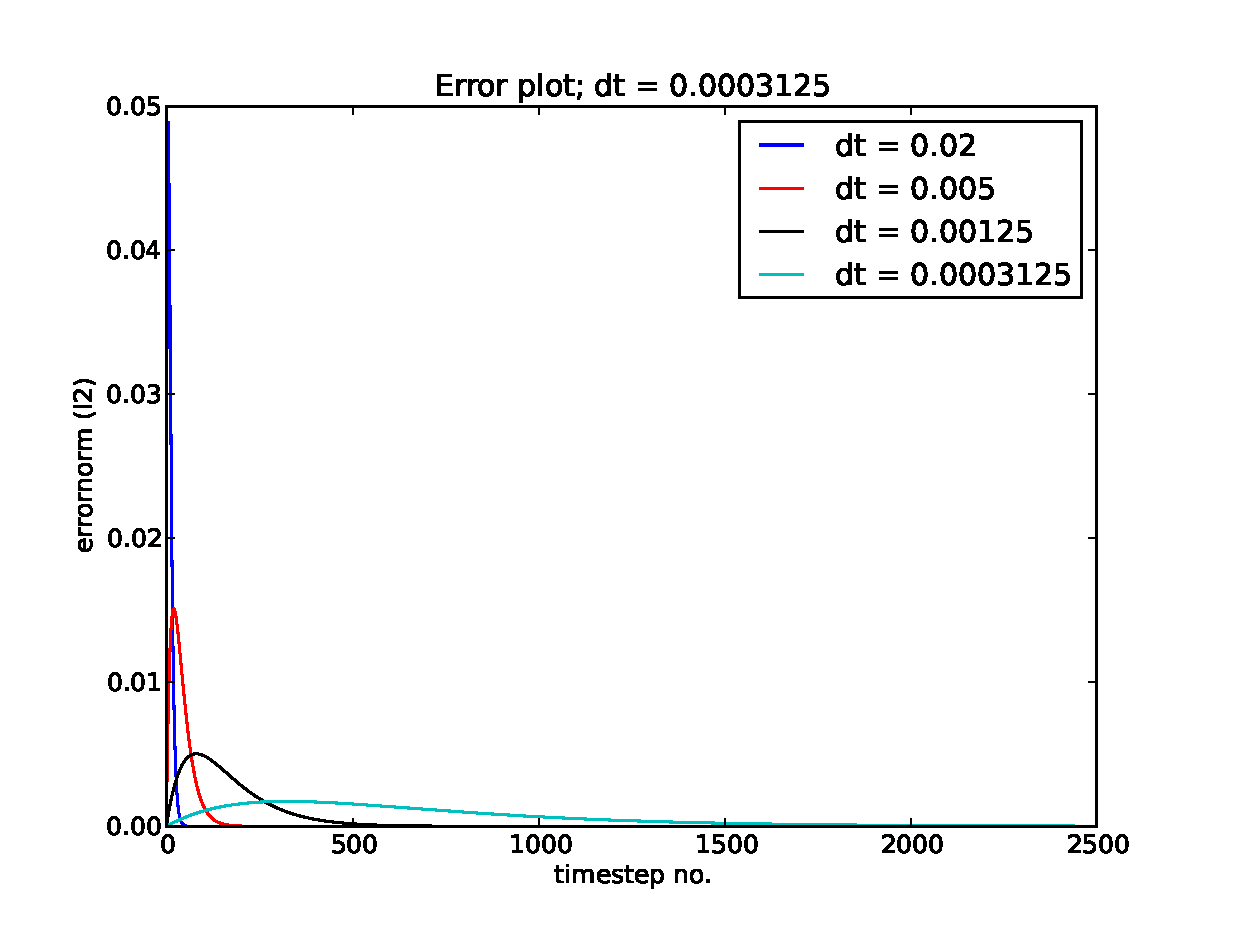
\includegraphics[width=\textwidth]{../results/experiment_18042014_1014_convergencetest_FE1D/results/errorplot.eps}
  \caption{}
 \end{subfigure}
 \begin{subfigure}{0.49\textwidth}
  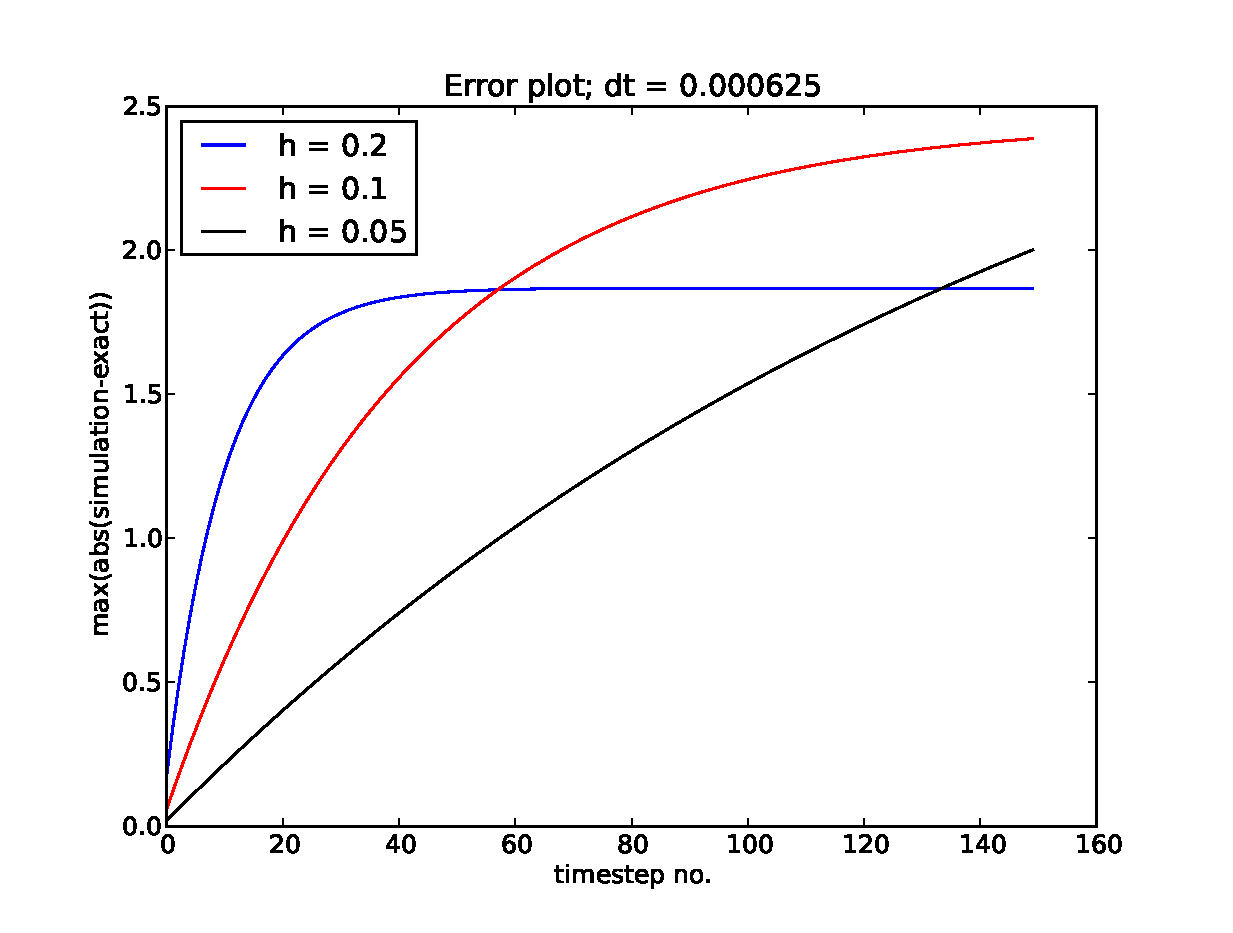
\includegraphics[width=\textwidth]{../results/experiment_29112013_1709/results/errorplot.eps}
  \caption{}
 \end{subfigure}
 \caption[]{}
 \label{analysis:errorplots:FE}
\end{figure}


\begin{figure}[h]
% Error plots for BE in 1D (a) and 2D (b)
\centering
 \begin{subfigure}{0.49\textwidth}
  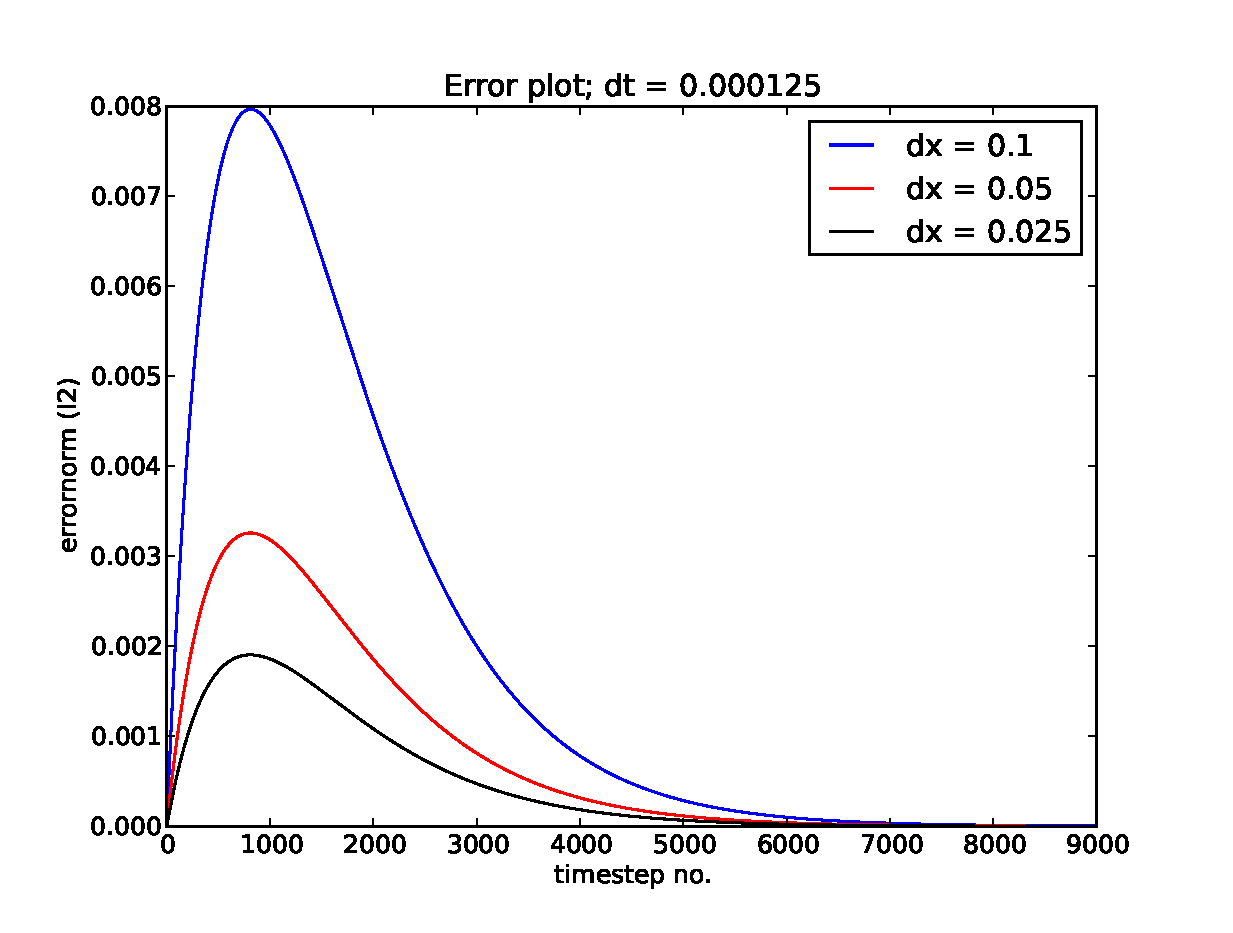
\includegraphics[width=\textwidth]{../results/experiment_14042014_1303_convergence_tests_etc/results/errorplot.eps}
  \caption{}
 \end{subfigure}
 \begin{subfigure}{0.49\textwidth}
  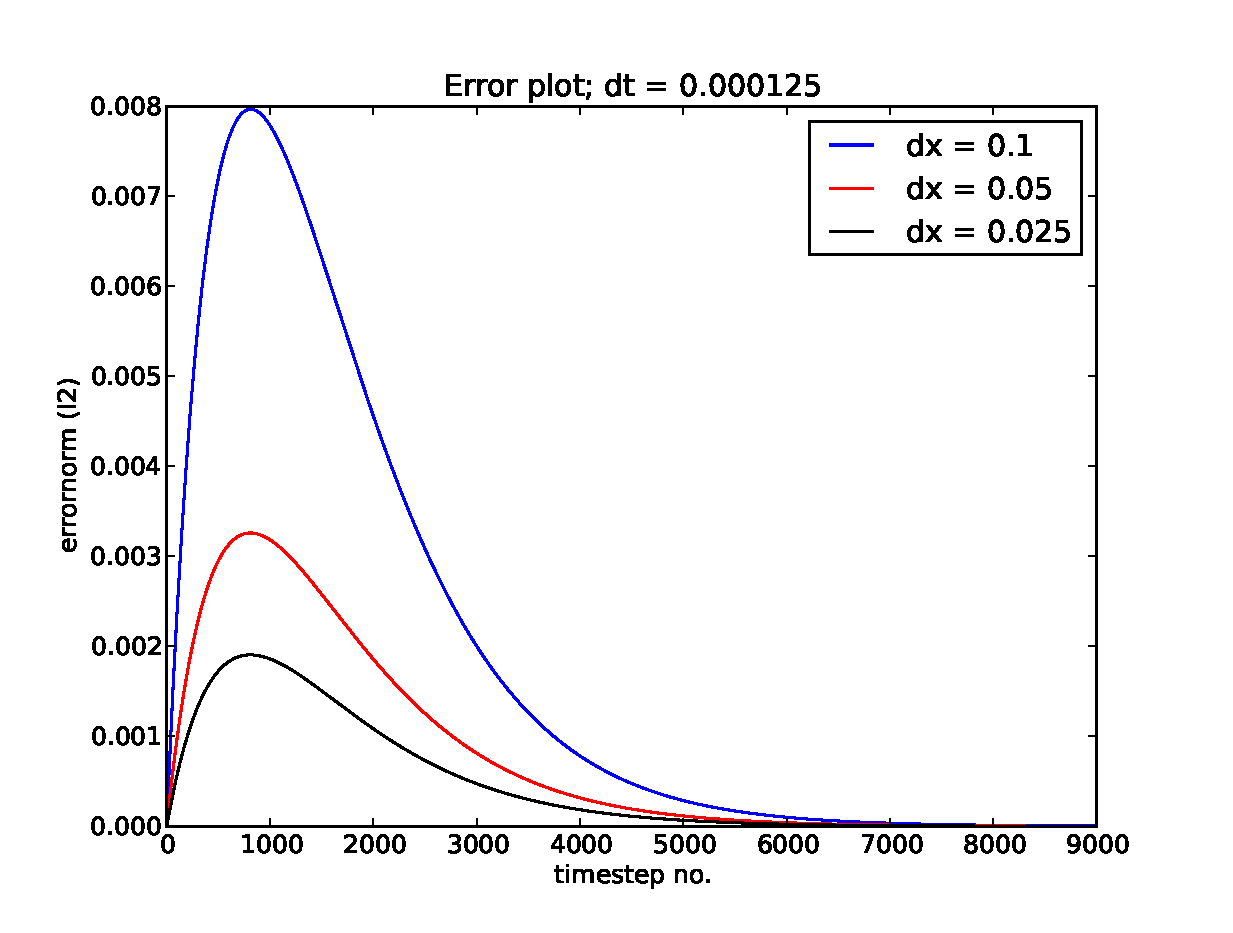
\includegraphics[width=\textwidth]{../results/experiment_14042014_1303_convergence_tests_etc/results/errorplot.eps}
  \caption{\emph{\textcolor{red}{This is not the correct plot!}}}
 \end{subfigure}
 \caption[]{}
 \label{analysis:errorplots:BE}
\end{figure}

\subsection{Verification by convergence tests}

The convergence tests are done by isolating the error term from either the time derivative or the spatial derivative, and refining the relevant discretization parameter over several simulations. 
Figures \ref{analysis:convergence_tests:FE} and \ref{analysis:convergence_tests:BE} verify that the error associated with the time derivative is of the expected order while figure \ref{analysis:spatial_convergence_test} verifies the error from the spatial derivative for the BE scheme.

\begin{figure}[h]
% Error plots for BE in 1D (a) and 2D (b)
\centering
 \begin{subfigure}{0.49\textwidth}
  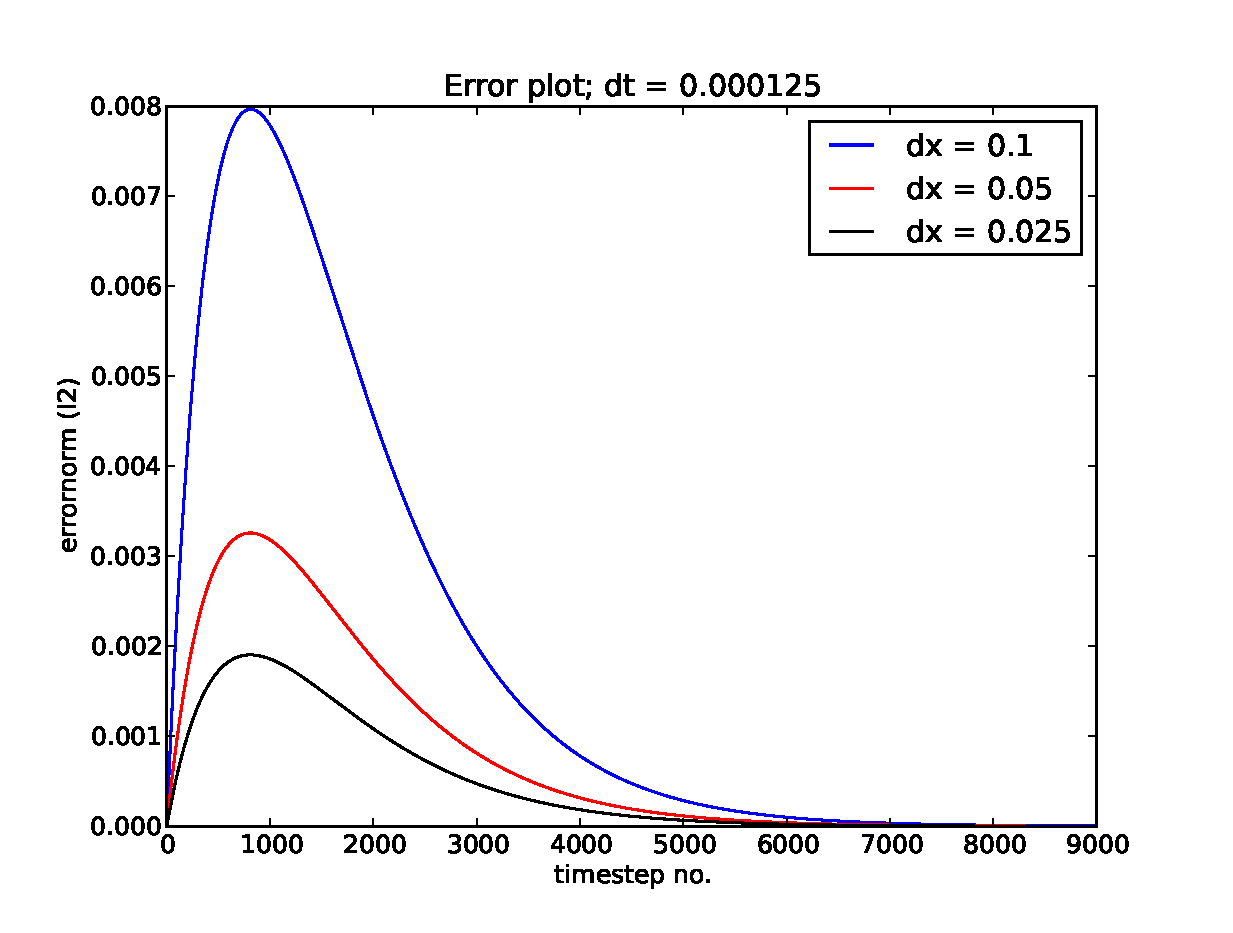
\includegraphics[width=\textwidth]{../results/experiment_14042014_1303_convergence_tests_etc/results/errorplot.eps}
  \caption{}
 \end{subfigure}
 \begin{subfigure}{0.49\textwidth}
  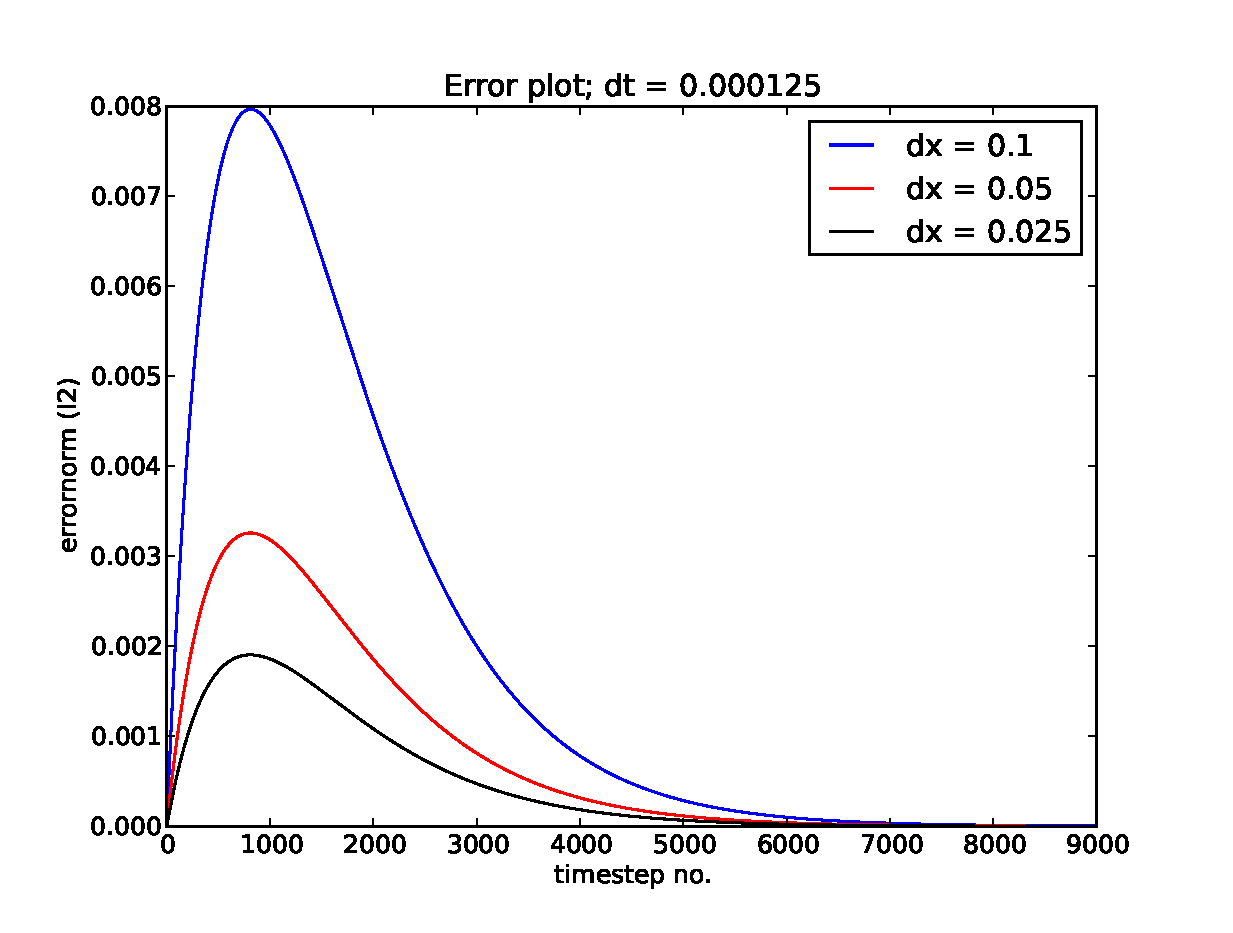
\includegraphics[width=\textwidth]{../results/experiment_14042014_1303_convergence_tests_etc/results/errorplot.eps}
  \caption{\emph{\textcolor{red}{This is not the correct plot!}}}
 \end{subfigure}
 \caption[]{}
 \label{analysis:convergence_tests:FE}
\end{figure}

\begin{figure}[h]
% Error plots for BE in 1D (a) and 2D (b)
\centering
 \begin{subfigure}{0.49\textwidth}
  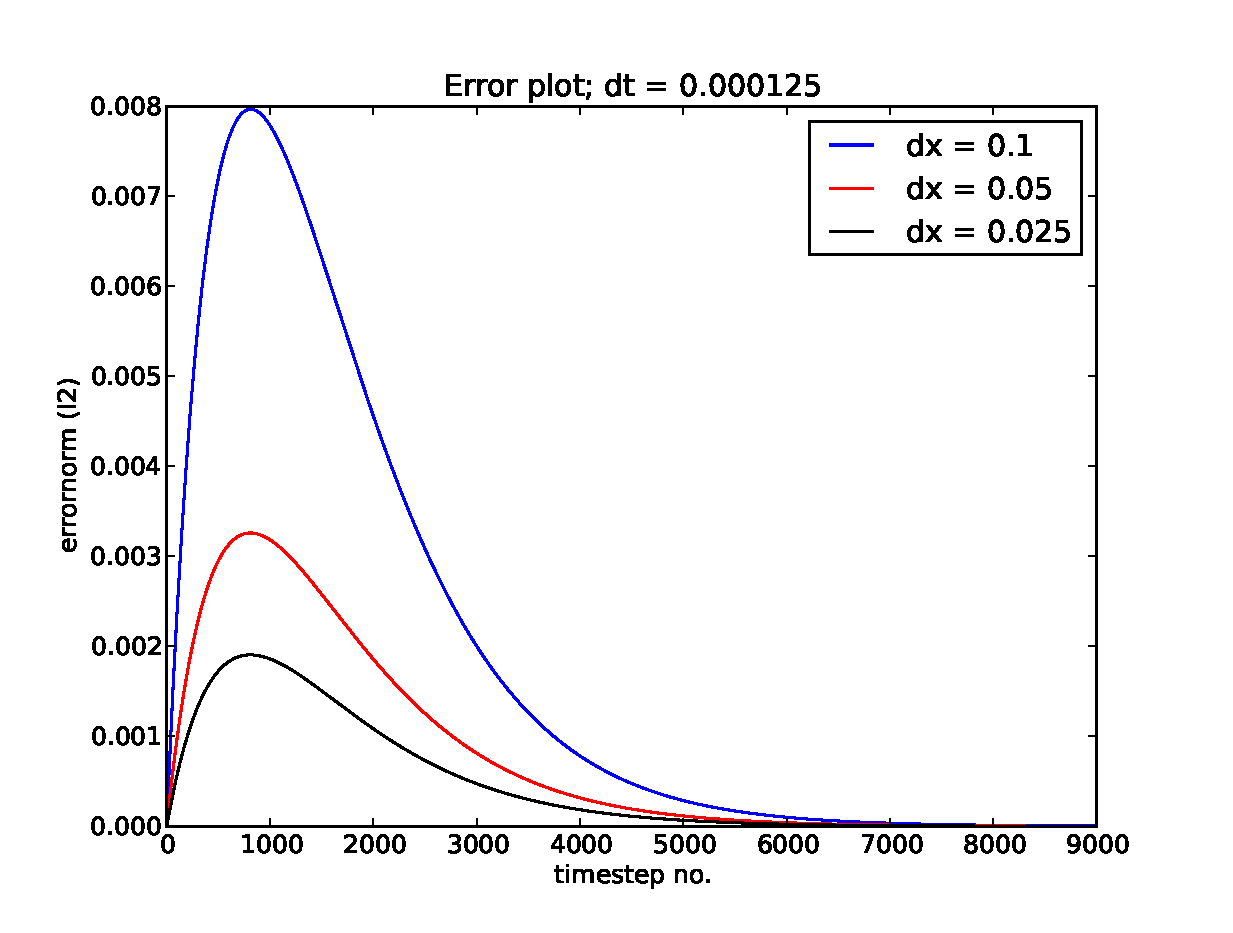
\includegraphics[width=\textwidth]{../results/experiment_14042014_1303_convergence_tests_etc/results/errorplot.eps}
  \caption{}
 \end{subfigure}
 \begin{subfigure}{0.49\textwidth}
  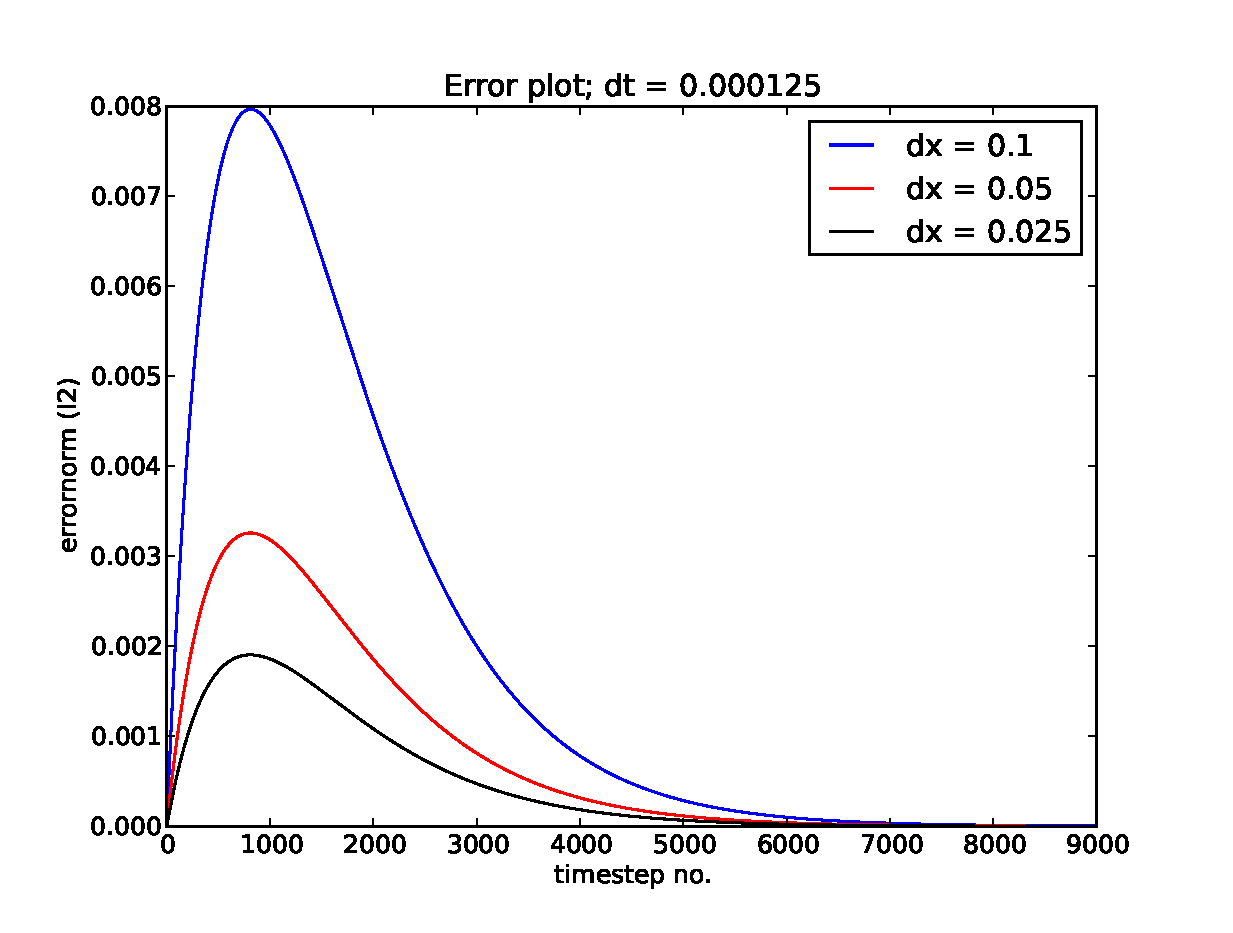
\includegraphics[width=\textwidth]{../results/experiment_14042014_1303_convergence_tests_etc/results/errorplot.eps}
  \caption{\emph{\textcolor{red}{This is not the correct plot!}}}
 \end{subfigure}
 \caption[]{}
 \label{analysis:convergence_tests:BE}
\end{figure}

\begin{figure}[h]
% Error plots for BE in 1D (a) and 2D (b)
\centering
 \begin{subfigure}{0.49\textwidth}
  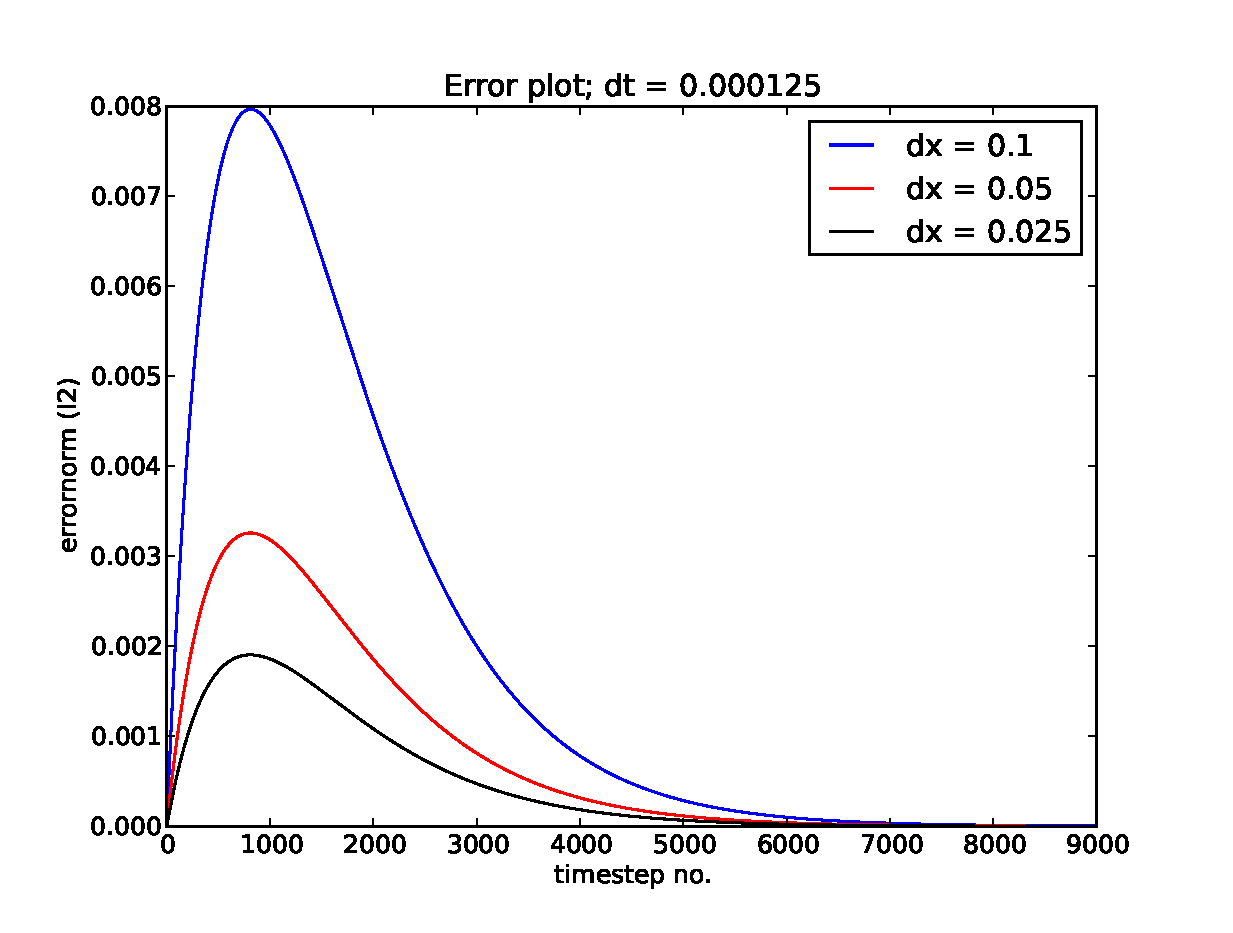
\includegraphics[width=\textwidth]{../results/experiment_14042014_1303_convergence_tests_etc/results/errorplot.eps}
  \caption{}
 \end{subfigure}
 \begin{subfigure}{0.49\textwidth}
  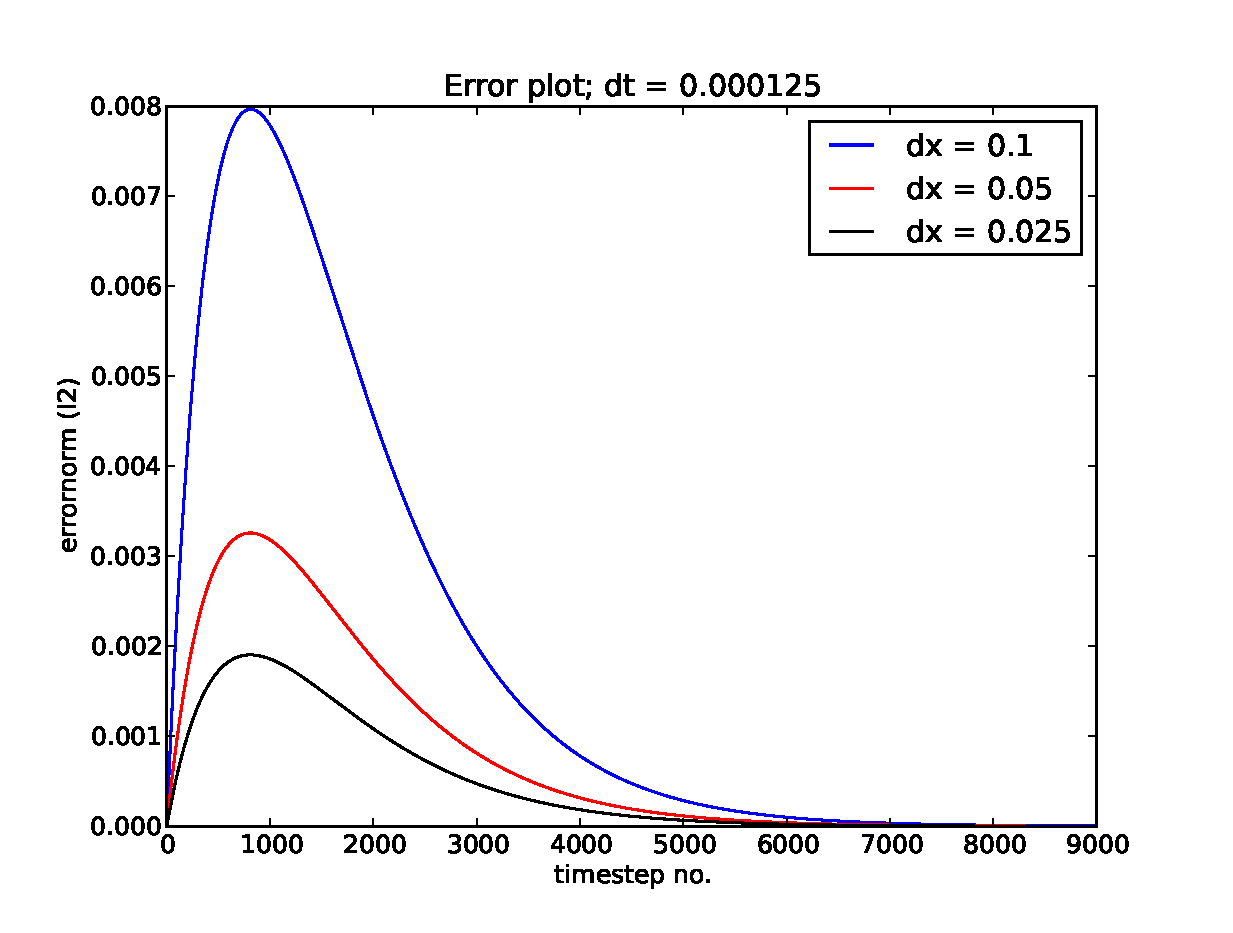
\includegraphics[width=\textwidth]{../results/experiment_14042014_1303_convergence_tests_etc/results/errorplot.eps}
  \caption{\emph{\textcolor{red}{This is not the correct plot!}}}
 \end{subfigure}
 \caption[]{}
 \label{analysis:spatial_convergence_tests}
\end{figure}
\subsection{Verification of FE scheme by exact numerical solution}

Discretization of the diffusion equation by the FE scheme yields the following numerical scheme in 1D
\begin{equation}
 u^{n+1} = D\Delta t u^n_{xx} + u^n
\end{equation}
where $u_{xx}$ denotes the double derivative of $u$ with respect to $x$. 
To illustrate how the equation is solved by the computer, the first four iterations are written out
\begin{align*}
 u^1 &= D\Delta t\, u_{xx}^0 + u^0 \\
 u^2 &= D\Delta t\, u_{xx}^1 + u^1 \\
 &= D\Delta t\left[D\Delta t u_{4x}^0 + u_{2x}^0\right] + u^0\\
 &= \left(D\Delta t\right)^2 u_{4x}^0 + 2D\Delta t u_{2x}^0+ u^0 \\
 u^3 &= D\Delta t\, u_{xx}^2 + u^2 \\
 &= D\Delta t\left[\left(D\Delta t\right)^2 u_{6x}^0 + 2D\Delta t u_{4x}^0+ u_{2x}^0\right] + \left(D\Delta t\right)^2 u_{4x}^0 + 2D\Delta t u_{2x}^0+ u^0\\
 &= \left(D\Delta t\right)^3 u_{6x}^0 + 3\left(D\Delta t\right)^2 u_{4x}^0+ 3D\Delta tu_{2x}^0 + u^0 \\
 u^4 &= D\Delta t \,u_{xx}^3 + u^3 = \dots \\
 &= \left(D\Delta t\right)^4 u_{8x}^0 + 4\left(D\Delta t\right)^3 u_{6x}^0+ 6\left(D\Delta t\right)^2 u_{4x}^0 + 4D\Delta t u_{2x}^0 + u^0 
\end{align*}

\noindent From the iterations above a pattern emerges for iteration $n+1$\\
\begin{equation}
 u^{n+1} = \sum\limits_{i=0}^n {n\choose i}\left(D\Delta t\right)^iu^0_{2ix}
\end{equation}
Where $u^0$ is the initial condition
\begin{equation}
 u^0 = \cos(\pi x)
\end{equation}
The spatial derivatives are found as
\begin{align*}
 u^0_{xx} &= \frac{1}{\Delta x^2}\left(\cos(\pi(x+\Delta x)) -2\cos(\pi x) +\cos(\pi(x-\Delta x))\right) \\
 &= \frac{2}{\Delta x^2}\left(\cos(\pi\Delta x)-1\right)\cos(\pi x)\\
 u^0_{4x} &= [u^0_{xx}]_{xx} \frac{1}{\Delta x^2}\left[\frac{u^0_{xx}}{\cos(\pi x)}\left(\cos(\pi(x+\Delta x)) -2\cos(\pi x) +\cos(\pi(x-\Delta x))\right)\right]\\
 &= \frac{4}{\Delta x^2}\left(\cos(\pi\Delta x)-1\right)^2\cos(\pi x)\\
 &\dots
\end{align*}
The pattern continues allowing the final numerical exact solution to be expressed in equation \eqref{numerical_solution}.
\begin{equation}\label{numerical_solution}
  u^{n+1} = \sum\limits_{i=0}^n {n\choose i}\left(D\Delta t\right)^i\frac{2^i}{\Delta x^{2i}}\left(\cos(\pi\Delta x)-1\right)^i\cos(\pi x)
\end{equation}

Although the FE scheme is expected to represent equation \eqref{numerical_solution} to machine precision ($\epsilon \approx 10^{-16}$) there are two problems with the solution which will have an effect on the error:
\begin{itemize}
 \item $\Delta x^{2i}$ will quickly tend to zero, and the computer will interpret it as zero. This will cause division by zero, which again results in ``Not a number'' (nan) and ruins the simulation. Testing if $\Delta x^{2i}>0$ and returning zero if the test fails will fix the problem. The argumentation for ignoring the troublesome terms is given below.
 \item ${n\choose i}$ goes to infinity for large $n$ and $i$. The computer can only represent numbers up to $\sim10^{308}$, which limits the number of steps to $170$ since $n!>10^{308}$ for $n>170$.
\end{itemize}

As a side note, equation \eqref{numerical_solution} illustrates how the stability criterion for the FE scheme comes into place. 
In the numerical exact solution the exponential which is found in the exact solution to the PDE (eq. \ref{manufactured_solution}) is replaced by an amplification factor $A^n$.
This amplification factor can be found in equation \eqref{numerical_solution} as 
\begin{equation}
A^n = \left(\frac{2D\Delta t}{\Delta x^2}\right)^i
\end{equation}
Inserting a time step larger than the stability criterion ($\Delta t \leq \frac{\Delta x^2}{2D}$) will make the amplification factor $A$ larger than one which in turn will make the solution blow up. \\
The stability criterion also illustrates why the terms where 
$$ \frac{1}{\Delta x^{2i}} \to \infty$$
 can be dropped. 
 By the stability criterion, the time step will cancel out $\Delta x^2$, and the result will be a number smaller than 1 raised to a rather large power, $i$, resulting in a number comparable to zero.\\
 
 The results from comparing a 1D simulation to the numerical exact is shown in Figure \ref{numerical_exact_FE:1D}. 
 As expected the error is larger than machine precision by at most two orders of magnitude because of accumulating error terms from the dropped terms in eq. \eqref{numerical_solution}.
 
 Using the same method as in the 1D case, a numerical exact solution can be found to the 2D FE scheme. 
 \begin{equation}\label{exact_numerical_solution_2d}
 u^{n+1} = \sum\limits^n_{i=0}{n\choose i}\left(D\Delta t\right)^i\left[2^{i-1}\cos(\pi x)\cos(\pi y)\left(\frac{(\cos(\pi\Delta x))^i}{\Delta x^{2i}} +\frac{(\cos(\pi\Delta y))^i}{\Delta y^{2i}}\right)\right]
\end{equation}

The same problems as in the 1D case will apply to equation \eqref{exact_numerical_solution_2d} with the same solutions. 
Figure \ref{numerical_exact_FE:2D} shows how the 2D simulation compares to the numerical exact solution. 
As was the case in 1D the error is larger than machine precision, but much smaller than $\Delta t$ suggesting that the scheme is implemented correctly.

\begin{figure}[H]
 \centering
 \begin{subfigure}{0.49\textwidth}
 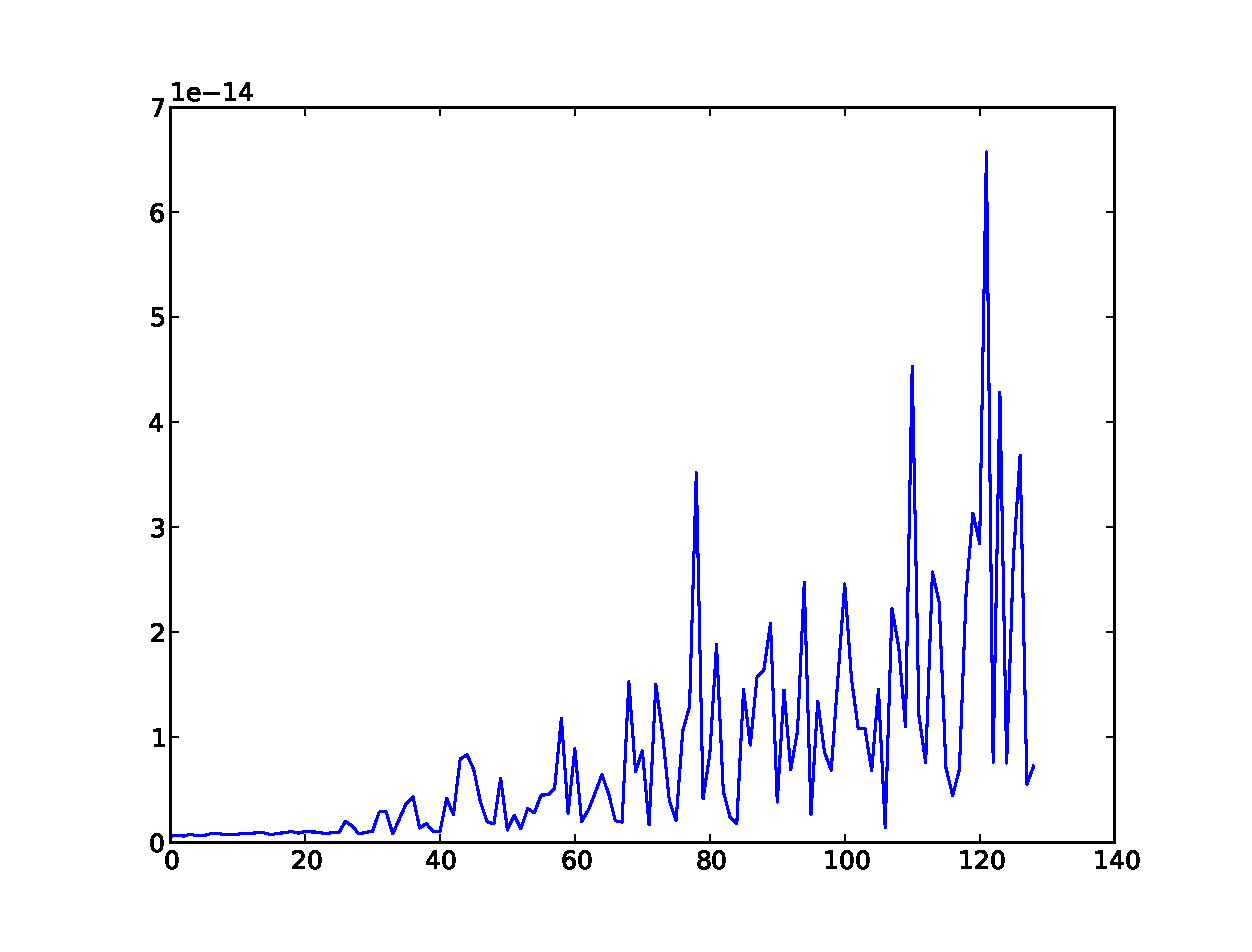
\includegraphics[width=\textwidth]{Figures/exact_numerical_1d_n130.eps}
  \caption{}
  \label{numerical_exact_FE:1D}
 \end{subfigure}
 \begin{subfigure}{0.49\textwidth}
 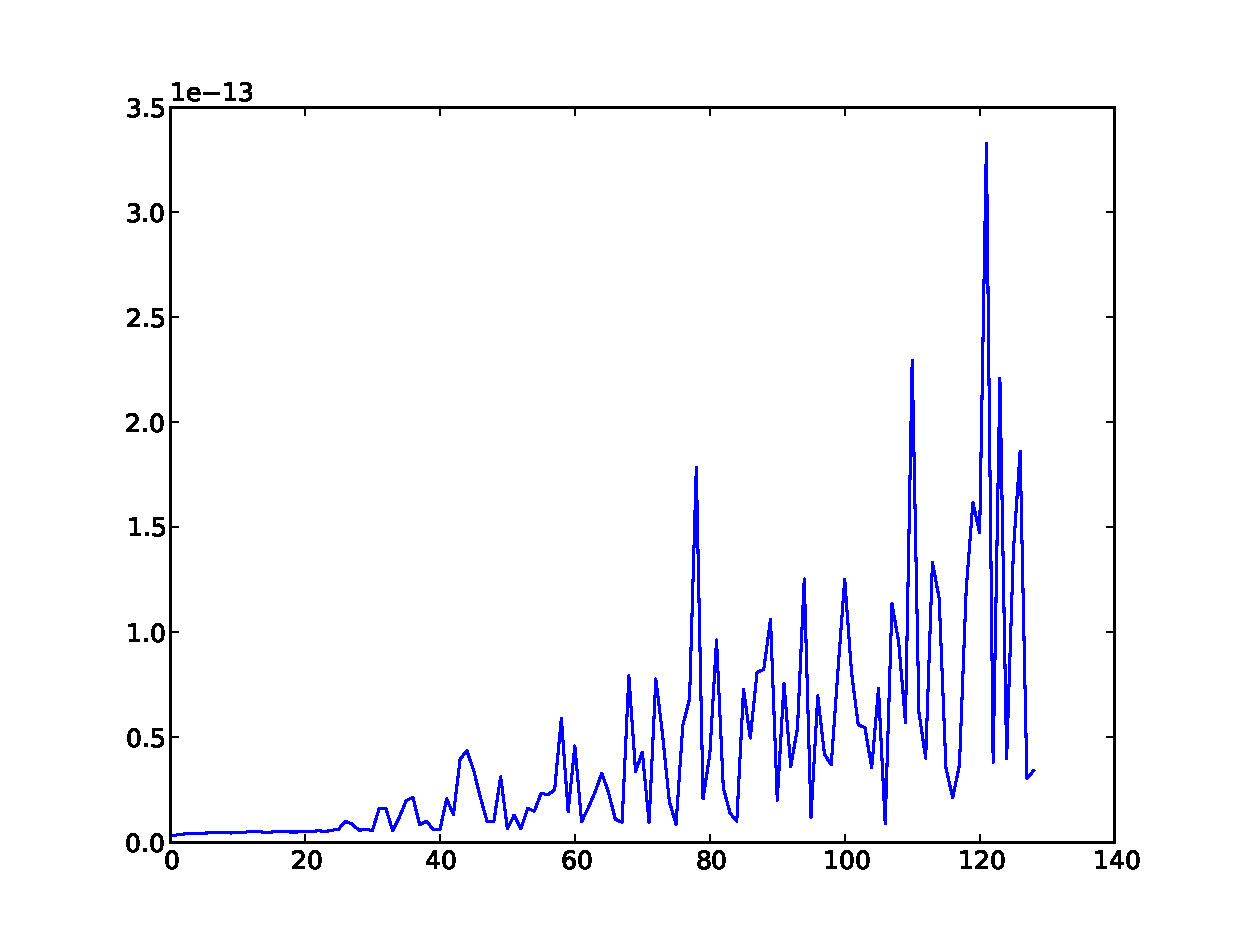
\includegraphics[width=\textwidth]{Figures/exact_numerical_2d_n130.eps}
  \caption{}
  \label{numerical_exact_FE:2D}
 \end{subfigure}
 \caption[Numerical exact error plots FE]{Numerical solution from the FE scheme in 1D (a) and 2D (b) versus the exact numerical solution of the FE scheme.
 Some of the terms in the numerical exact solutions are ignored to prevent overflow and this is responsible for the increasing error which is slightly larger than machine precision.}
 \label{numerical_exact_FE}
\end{figure}


\subsection{Verification of BE scheme by exact numerical solution}

The exact numerical solution to the BE scheme is found by solving the linear system which arises from the discretization. 
\begin{align*}
 \mathbf M \mathbf u^{n+1} &= \mathbf{u}^n \\
 \mathbf{u}^{n+1} &= \mathbf{M}^{-1} \mathbf{u}^n \\
 &= \mathbf{M}^{-1}\left(\mathbf{M}^{-1} \mathbf{u}^{n-1}\right)
\end{align*}

Doing the separation to the end relates the $n$'th time step to the initial condition
\begin{equation}\label{BE_numex}
 \vec u^{n+1} = \left(\mathbf M^{-1}\right)^{n+1} \vec u^0
\end{equation}

Note that $\left(\mathbf M^{-1}\right)^{n+1}$ is the inverse of $\mathbf M$ to the $n+1$'th power.\\

Taking the inverse of $\mathbf M$ will result in a dense matrix where a lot of the entries are close to zero (e.g. $10^{-20}$). 
Doing calculations with such a matrix gives a lot of round off errors which will reduce the accuracy of the numerical exact. 
The error should theoretically be machine precision, but is expected to at least be much smaller than $\Delta t$. 
Errors from both 1D and 2D simulations are shown in Figure \ref{numex:BE_errorplot}

\begin{figure}[H]
 \centering
 \begin{subfigure}{0.49\textwidth}
 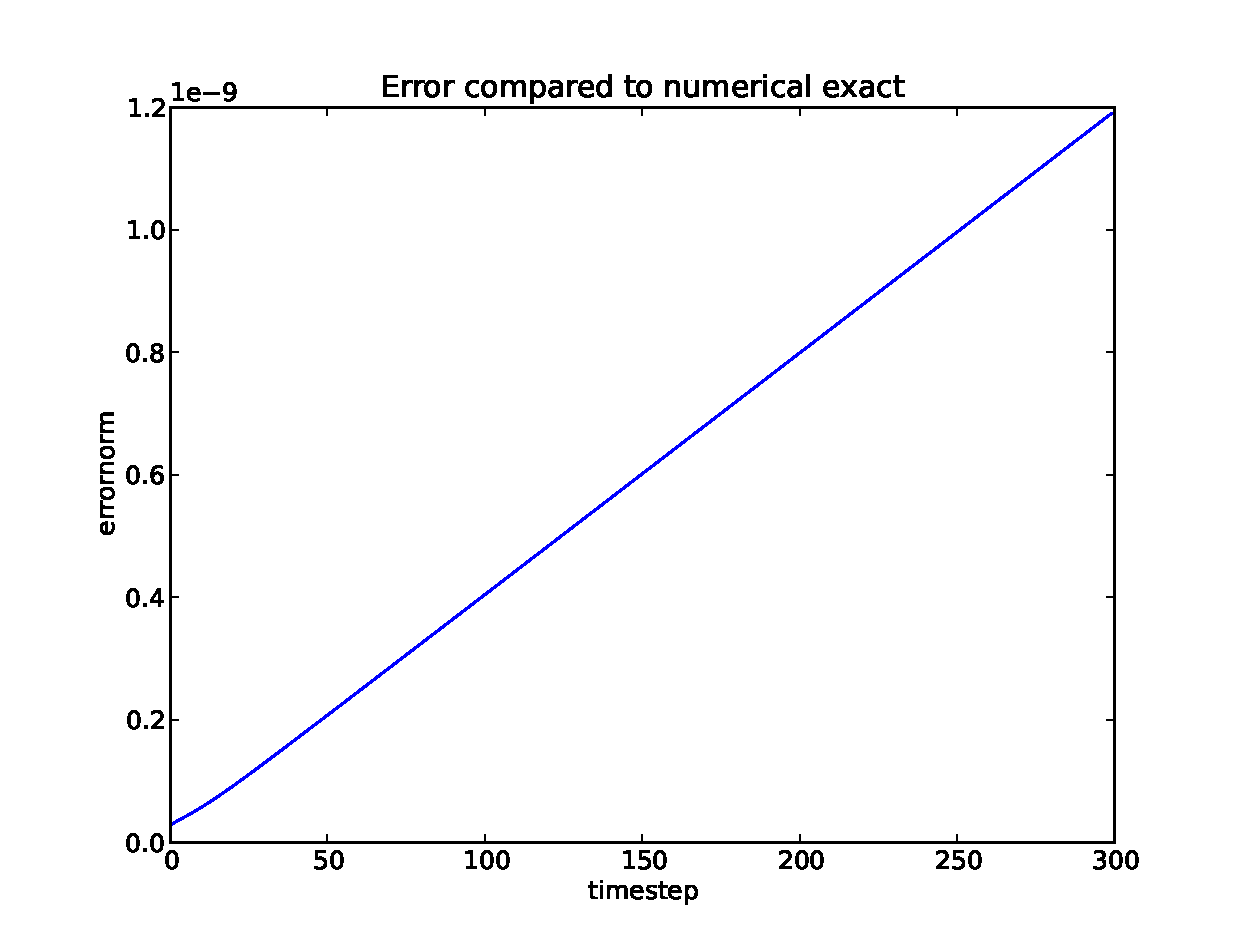
\includegraphics[width=\textwidth]{../results/experiment_14042014_0759_BE1D_numerical_exact/results/numerical_exact.eps}
 \caption{}
\end{subfigure}
\begin{subfigure}{0.49\textwidth}
 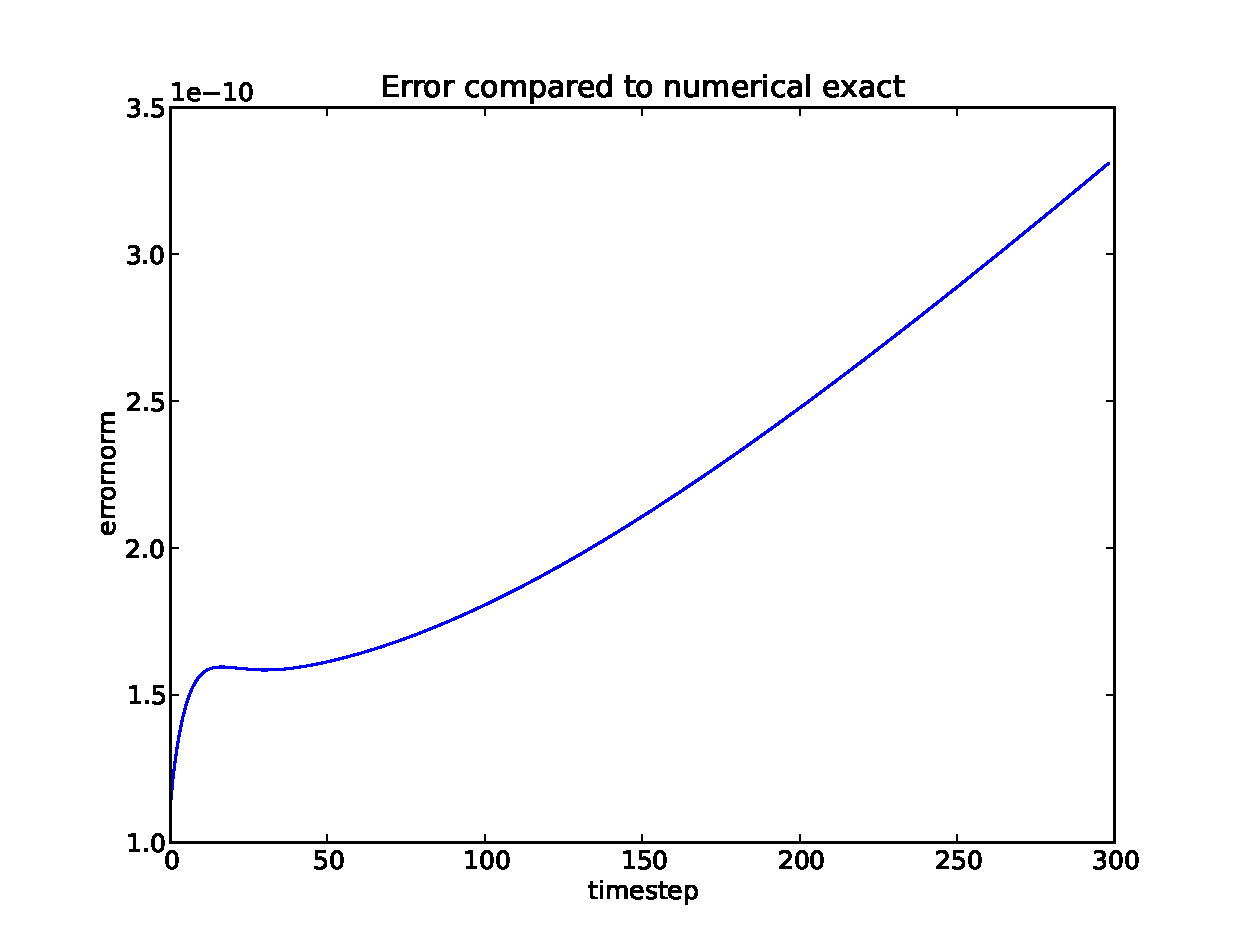
\includegraphics[width=\textwidth]{../results/experiment_30042014_0914_BE2D_numex/results/numerical_exact.eps}
 \caption{}
\end{subfigure}
 \caption[Numerical exact errorplots for BE scheme]{Plots showing the error for the BE scheme in 1D (a) and 2D (b) compared to the numerical exact solution. 
 The error is not machine precision, but significantly smaller than $\Delta t$ which for these simulations is $\Delta t=0.01$. 
 This increased error originates in the many roundoff errors in the inverted matrix where a lot of terms $10^{-16}$ and smaller.}
 \label{numex:BE_errorplot}
\end{figure}

\section{Verification of the RW solver}


\chapter{Physical application}\label{chapter:application}
\clearpage
The following chapter is included to show that the developed hybrid diffusion solver can be applied to real life problems with only minor modifications.

\section{Physical scope}


\emph{\textcolor{red}{Her bør det stå noe om hva vi holder på med og hvor det kommer fra, samt hvorfor det er interessant og hva vi faktisk kommer til å måle (diffusjonstid for walkers gjennom spine neck).}}

PKC$\gamma$ is associated with memory storage and will diffuse out of the cell body (soma) of a neuron through a dendrite into a dendritic spine to reinforce the absorption of neurotransmitters. 
This application is aimed at modeling PKC$\gamma$ diffusion in a dendrite and into spines. 
Because of symmetry the dendrite will be modeled as 1D continuous diffusion while the diffusion in spines will be modeled as a random walk. 
Effectively we will investigate the diffusion time for random walkers through spine necks which are very narrow ($\leq0.5\mu$m). 
The results will be compared to results by Craske et.al \cite{craske2005spines}.

\section{Implementation}

There is a difference between the approach of the developed hybrid solver and the dendrite - spine system with respect to geometry which is best summarized in figure \ref{application:geometry_difference}.

\begin{figure}[H]
 \centering
 \begin{subfigure}{0.48\textwidth}
  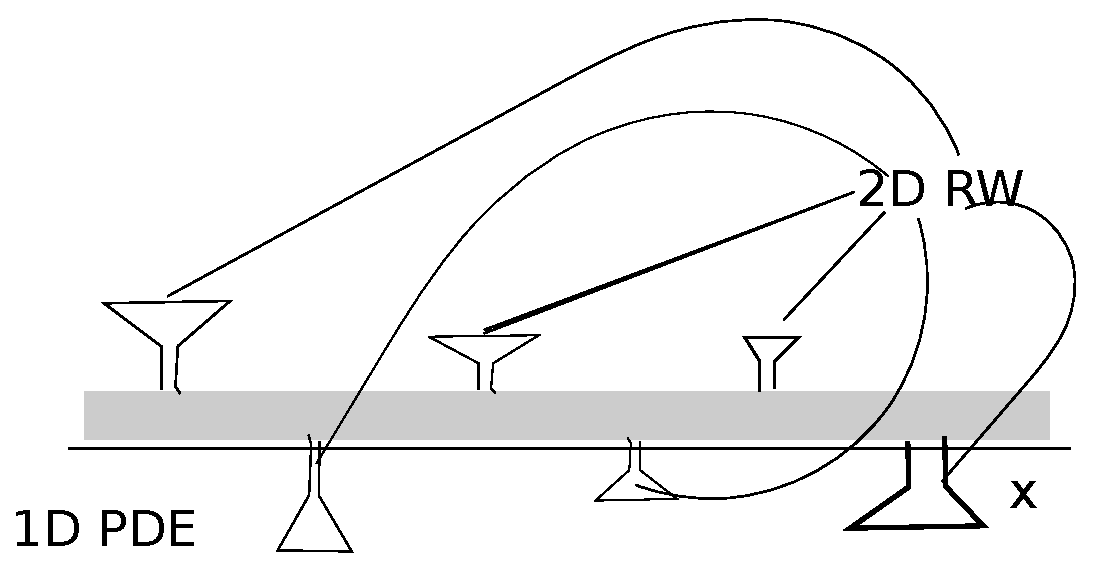
\includegraphics[width=\textwidth]{Figures/dendrite_spine_model.eps}
  \caption{}
 \end{subfigure}
 \begin{subfigure}{0.48\textwidth}
  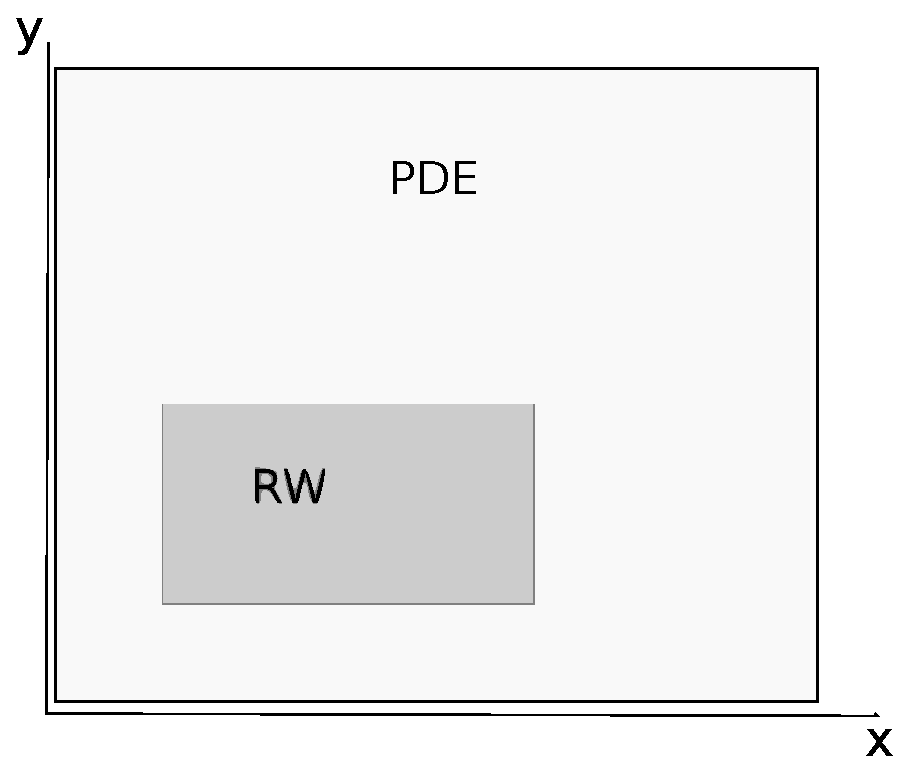
\includegraphics[width=\textwidth]{Figures/hybrid_model_principle.eps}
  \caption{}
 \end{subfigure}
 \caption[Difference between hybrid diffusion solver and dendrite - spine diffusion model]{The geometric difference between the original hybrid diffusion solver (b) and the problem of PKC$\gamma$ diffusing into dendritic spines (a). }
 \label{application:geometry_difference}
\end{figure}

The hybrid diffusion solver has been slightly modified in order to recreate the new geometry. 
Mathematically the largest difference is that the random walkers are left alone, meaning that the diffusion equation is not solved in the spines. 
There are also some differences in the coupling; at each PDE time step there is a probability for an enzyme to diffuse into a spine if the concentration at the beginning of the spine neck is large enough. This probability decreases with the number of enzymes which have already diffused into the spine. 
The width of a spine neck is determined by the number of PDE mesh points it connects to, all other length parameters are determined randomly but required to fit with measurements from Arrelano et.al \cite{arellano2007ultrastructure}. 

\subsection{Initial Condition}

In the presence of glutamate the diffusion constant for PKC$\gamma$ has been measured to $0.33\frac{\mu m^2}{s}$, but this does not reproduce the diffusion times in dendrites which are illustrated by Craske et.al. 
There are two possible fixes to this; \emph{\textcolor{red}{either I have read the paper wrong, and the diffusion constant is really $5.72$ in the dendrite, in which case everything is ok.}} 
The other possibility is to modify the initial condition. The latter is not as far fetched as is sounds because there is considerable absorption of PKC$\gamma$ in the dendrite walls during the first few seconds after release from soma. 
The modified initial condition can be viewed as the concentration distribution in the dendrite some 2 seconds after release from soma.
\clearpage

\section{Parameters}

The new problem requires the introduction of some additional parameters as well as a reformulation of limiting factors for some known parameters, all of which are described in the following table.
 
 \begin{table}[H]
\centering
\begin{tabular}{|p{0.13\textwidth}|p{0.21\textwidth}|p{0.18\textwidth}|p{0.37\textwidth}|}
\hline
\textbf{Parameter} & \textbf{Explanation} &\textbf{Expression/ typical value}& \textbf{Origin} \\
\hline
$\Delta t$ & time-step & $\Delta x^2$ & stability criterion FE scheme \\
\hline
$\Delta x$ & spatial resolution & $\frac{1}{2}$min(spine neck diameter) & estimated \\
\hline
$Hc$ & conversion factor & 5-24 & estimated by calculations of concentration levels taken from \cite{light1996protein} and spine/dendrite volume ratios. See later for discussion. \\
\hline
$u(t=0)$ & initial condition value & 5$\frac{\text{nMol}}{\text{L}}$ & estimated from values found in \cite{light1996protein}\\
\hline
$p_{ds}$ & probability to diffuse into a spine & $0.1\cdot\Delta x\cdot\Delta t$& estimated. An important ability of this parameter should be that wide necked spines have larger probability and that a certain flux is maintained (on average), meaning that the flux should be independent of $\Delta t$ \\
\hline
$p_{ab}$ & probability for PKC$\gamma$ to be absorbed, and removed from simulation, per time-step taken in spine head & 100\% & estimated\\
\hline
\end{tabular}
\caption[Important parameters]{Parameters which play an important role in the simulation of PKC$\gamma$ diffusion into dendritic spines with explanations, expressions/typical values and an indication as to where the value/expression has its origin.}
\label{table:parameters}
\end{table}


\chapter{Results}
\clearpage
\section{Validity of the model}
The results of the testing done in the Analysis-chapter, particularly the convergence tests based on varying the conversion-factor, Hc, to exceed the expected numerical error arising from the scheme itself based on equation \ref{}, suggest that the implementation of our model is correct. 
The mathematics overlap, as we have seen in chapter \ref{}, and if we introduce enough walkers there seems to be no difference between adding an area on the mesh where random walks solve the equation, and not doing so. 
In other words, our model converges to the continuum model in the limit of sufficient walkers.

\chapter{Discussion and conclusion}
\clearpage
\section{Discussion}

A large portion of the work that has been put into this thesis has been on code implementation. 
Because it is really demanding to read computer code, and it does not necessarily provide extra clarity, the code is not included in this text. 
Should it be of interest, the complete computer code is published at github.com under the following link\\

\noindent\url{https://github.com/fepettersen/thesis} \\



\subsection{Other work on the subject}

As the project was being finished, I came across an article by Flekkøy et.al.\cite{flekkoy2001coupling} describing the same problems that are addressed in this thesis. 
In this article, the authors try to combine a simple diffusion solver with a simple random walk solver and end up concluding that this is possible. 
This thesis has been done completely independently of said article, and takes a slightly different approach to the problem as well.

\subsection{Application}

The model gives fairly good results for the application on PKC$\gamma$ into spines which largely are in agreement with the results by Craske et.al. 
However, the mean diffusion times found from simulations seem to consistently lie towards the lower limits of the experimental results. 
One possible extension to the model which might fix this is to introduce an absorption probability in the spine head which is fairly large (say 80\% per second), or even increases with the amount of time spent in the spine head. 
A setup like this should increase the average diffusion time by a few seconds. 
It does not, however reflect the physical process to a better accuracy seeing as a concentration increase in a spine head will be measured quickly.

\subsection{Alternatives to the implemented PDE solver}
% \subsection{Higher order approximations to the time derivative}
Although a first order approximation to the time derivative might seem primitive, the aim of this thesis was to prove the concept of combining two different models for the same problem. 
For verification purposes, the demand for walkers is already very high, at
\begin{equation*}
 Hc \geq \frac{1}{\Delta t^2}
\end{equation*}
In order to carry out the same verification for a second order scheme, the demand for walkers will become much larger
\begin{equation*}
 Hc \geq \frac{1}{\Delta t^4}
\end{equation*}

For future use, however, the concept has already been proven, and a higher order scheme would be an interesting, yet simple extension.

Perhaps the biggest weakness of the software, as it stands, is the limitation in mesh geometry. 
% The mesh must be quadratic
Implementing a mesh geometry which is not square in a finite difference method turns out to be very complicated, and requires transforming the PDE to a new set of coordinates. 
Ultimately one must solve an entirely different equation. 
Alternatively, a finite element method can be used. 
Finite element software will already have support for new mesh geometries built in, making the suggested transformations unnecessary.

\subsection{The lower scale model}

A simple RW was chosen for the lower scale model because it fulfills the diffusion equation and is therefore easy to work with. 
The idea, however, was always to create a software in which the lower scale model can easily be substituted for a better one. 
By letting the lower scale model work as a standalone unit which communicates with the rest of the software through a file containing the positions of all the walkers (or particles), this is ensured. 
All that is needed to switch lower scale model is to put the new solver in the correct place with respect to the rest of the software, and make sure it can communicate in the described manner. 
As a test, the DSMC code developed by Anders Hafreager was used as a lower scale model for one simulation. 
Naturally, a few problems arise, but from a strictly programming point of view it worked. \\

As mentioned in section \ref{theory:BC_RW}, perfect flux exchange between the higher and lower scale model might have been a better boundary condition for the RW model than zero flux boundary conditions. 
I principle, changing boundary conditions on the RW solver is simple, seeing as it is completely separate from the rest of the software. 
The reason the boundary conditions have not been changed is that it requires a complete workover of the coupling between the two models as well, which is a much larger job. 



\section{Conclusion}

In this thesis a hybrid diffusion solver in which parts of the process can be modeled by a particle dynamics description has been developed. 
All parts of the solver have been verified to work properly, including the hybrid model. \\


The developed software mainly relies on the implicit BE scheme to solve the diffusion equation, both in 1D and in 2D. 
Like any implicit scheme, the BE scheme results in a system of linear equations of size $n^d\times n^d$ which must be solved at each time step. 
In order to do so, a block tridiagonal solver has been implemented, with an efficiency of $\mathcal{O}(n^{2d-1})$. 
To my knowledge, this is the most effective direct solver available, with alternatives like LU decomposition and Levinson recursion using $\mathcal{O}(n^{2d})$ FLOPs. 
The limiting factor of the block tridiagonal solver is two matrix-vector multiplications which will use $\mathcal{O}(n^{2(d-1)})$ FLOPs. 
If a faster matrix-vector multiplication scheme exists it will reduce the computational work to $\mathcal{O}(n^d)$. \\



\appendix
\chapter{Appendix}
\section{Various calculations}

In this appendix some more tedious and rather boring, but no less important calculations can be found. 
We will also list some algorithms that are important, but not quite in the scope of this thesis.

\subsection{Backward Euler scheme in 2D}

Using the BE discretization on the simple 2D diffusion equation will yield the general scheme in equation \ref{general_scheme_BE2D}.
\begin{equation}\label{general_scheme_BE2D}
 u^{n}_{i,j} = \underbrace{\frac{-D\Delta t}{\Delta x^2}}_{\alpha}\left(u^{n+1}_{i+1,j}+u^{n+1}_{i-1,j}\right) +
 \underbrace{\left(1+\frac{2D\Delta t}{\Delta x^2} +\frac{2D\Delta t}{\Delta y^2}\right)}_{\gamma}u^{n+1}_{i,j} 
 \underbrace{-\frac{2D\Delta t}{\Delta y^2}}_{\beta}\left(u^{n+1}_{i,j+1}+u^{n+1}_{i,j-1}\right)
\end{equation}
This can, again, be written as a linear problem where the vectors are simply the matrices $u^n$ and $u^{n+1}$ written as column vectors. 
The matrix is written out for a $3\times3$ grid with no-flux Neumann boundary conditions in equation \ref{linear_system_BE2D}. 
We see that it is a five-band diagonal matrix, and so the tridiagonal solver cannot be used in this case. It is fully possible to use for example a Gaussian elimination in order to solve this equation, but it will require $\frac{2}{3}\mathcal{O}(n^3)$ operations per time step, where n is the size of the matrix (in this case $n=9$). 
Another way to solve this equation, and by extension use the BE scheme, is to use some form of sparse LU decomposition.
\begin{align}\label{linear_system_BE2D}
  \left(\begin{array}{c c c c c c c c c}
        \gamma & -2\beta &0 &-2\alpha &0 &0 &0 &0 &0\\
        -\beta & \gamma & -\beta &0 &-2\alpha &0 &0 &0 &0\\
        0&-2\beta & \gamma & 0 & 0 & -2\alpha &0&0&0\\
        -\alpha& 0&0 & \gamma & -2\beta & 0 & -\alpha &0&0\\
        0& -\alpha&0&-\beta & \gamma & -\beta & 0 & -\alpha &0\\
        0& 0& -\alpha&0&-2\beta & \gamma & 0 & 0 &-\alpha\\
        0& 0 &0 &-2\alpha &0&0 & \gamma & -2\beta&0\\
        0& 0 &0 &0 &-2\alpha&0&-\beta & \gamma &-\beta\\
         0&0 &0 &0&0 &-2\alpha&0&-2\beta & \gamma
       \end{array}\right)\mathbf{u}^{n} = \mathbf{u}^{n+1}
\end{align}
When we try to implement Neumann boundary conditions for grids that are larger than $3\times3$ we come across a problem. 
Doing the matrix-vector multiplication in equation \ref{linear_system_BE2D} reproduces the BE scheme with boundary conditions perfectly. 
However, if we extend to a $4\times4$ grid using a matrix on the same form we will start producing equations which will not arise from the scheme. 
This is illustrated in eqs. \ref{first_eq_BE2D_scheme} and \ref{first_eq_BE2D_linear_system}. 
Moving the off-diagonal entries with $\alpha$ one more column to the right and left will solve the problem, but this will force us to use some more general solver of a sparse linear system. 
All in all we will probably be better off using another scheme (at least in 2D).\\
The first equation that arises from the BE scheme in 2D (where $i=j=0$) is
\begin{equation}\label{first_eq_BE2D_scheme}
 u^n_{0,0} = \gamma u^{n+1}_{0,0}-2\alpha u^{n+1}_{1,0} -2\beta u^{n+1}_{0,1}
\end{equation}
while the first equation produced by the linear system in the $4\times4$ case is 
\begin{equation}\label{first_eq_BE2D_linear_system}
 u^n_{0,0} = \gamma u^{n+1}_{0,0}-2\alpha u^{n+1}_{0,3} -2\beta u^{n+1}_{0,1}
\end{equation}
which is an equation that will never be produced by the BE scheme. 
In the $3\times3$ grid-case the off-diagonal matrix entries with $\alpha$ are on the third column before and after the diagonal. 

Moving the corresponding entries to the fourth column in the $4\times4$ case, and similarly to the n'th column in the $n\times n$ case will fix the problem, but also increase the complexity of the matrix seeing as it will be $n+2$ band diagonal.\\
Extending the model to three spatial dimensions gives a very similar matrix to the 2d-case. 

\begin{align}\label{BE3D_linear_system}
  \left(\begin{array}{c c c c c c c c c}
        D_{00} & -2\beta I &0 &-2\alpha I &0 &0 &0 &0 &0\\
        -\beta I & D_{01} & -\beta I &0 &-2\alpha I &0 &0 &0 &0\\
        0&\ddots & \ddots & 0 & 0 & \ddots &0&0&0\\
        -\alpha I& 0&0 & D_{10} & -2\beta I& 0 & -\alpha I &0&0\\
        0& \ddots&0&\ddots & \ddots & \ddots & 0 & \ddots &0\\
        0& 0 &0 &-2\alpha I &0&0 & D_{n0} & -2\beta I&0\\
        0& 0 &0 &0 &\ddots&0&\ddots & \ddots &\ddots\\
         0&0 &0 &0&0 &-2\alpha I&0&-2\beta I & D_{nn}
       \end{array}\right)
       \left(\begin{array}{c}
             u^{n+1}_{00k}\\
             u^{n+1}_{01k}\\
             \dots\\
             u^{n+1}_{10k}\\
             \dots\\
             u^{n+1}_{n0k}\\
             \dots\\
             u^{n+1}_{nnk}
             \end{array}\right) = \mathbf{u}^{n}
\end{align}
In equation \ref{BE3D_linear_system} $I$ denotes the $n\times n$ identity, $D_{ij}$ denotes the tridiagonal $n\times n$ matrix with entries similar to the ones in eq. \ref{general_scheme_BE2D}, and off-diagonal entries similar to the ones in eq. \ref{general_scheme_BE2D}. 
All $0$'s denote the $n\times n$ zero-matrix. The values $\alpha$ and $\beta$ are the relevant coefficient matrices for the calculations in question. These will be diagonal as well (or simply numbers in the isotropic case). 
Note also that the vector entries $u^{n+1}_{ijk}$ are column vectors, making the vector $\mathbf{u}^{n+1}$ have the shape $1\times n^3$.

% \caption{Algorithm for Gaussian elimination of a tridiagonal linear system.}
% \label{tridiag}

\section{Alternatives to Random walks}
This section will mention some alternatives to the random walk model used in this project and discuss how realistic they are to combine with a diffusion PDE as one goal in this project has been. 
Both applications towards computational neuroscience and more general applications will be discussed. \\
These models are pretty complex with many details, and this project does not in any way try to do more than introduce them. 
Further reading is cited in the end of each section.

\subsection{Molecular Dynamics}
Molecular dynamics is the simulation of the dynamics of atoms and molecules using classical, Newtonian mechanics in the sense that the molecules are affected by a potential, and that the sum of forces describes the dynamics. 
Their dynamics are then integrated forward in time, and used to describe for example flow in nanoporous media. 
This means that the system is fully described by the position and velocities of all the atoms. 
Of course, there is a vast variety in the level of complexity here and we will only look at the simplest example, namely the Lennard-Jones potential, eq. (\ref{LJ}). 
This potential consists of an $r^{-12}$ term which denotes the Pauli repulsion at short ranges, and an $r^{-6}$ long range, attractive Van Der Waals term. 
The relative distance between two atoms is denoted by $r$. 
The Lennard-Jones potential is derived to simulate Argon in the Van Der Waals equation of state.
\begin{equation}\label{LJ}
 U = 4\epsilon\left[\left(\frac{\sigma}{r}\right)^{12}-\left(\frac{\sigma}{r}\right)^{6}\right]
\end{equation}
It is possible to do simulations of flow in nanoporous materials using the Lennard-Jones potential, although it is a far from perfect model, by only allowing some of the atoms to move. 
This will result in a matrix of stationary atoms, simulating a wall (note that there will still be forces acting from these atoms), and a liquid inside this matrix. \\

There are two main problems with using molecular dynamics more or less regardless of the application: 
It requires a potential which describes the forces working on all molecules in the simulation. 
This part may be particularly difficult when it comes to modeling macromolecules like proteins.\\
It might be really difficult to create the desired geometry for a simulation. 

For diffusion purposes this model is extremely temperature dependent, and not directly transferable to the diffusion processes described in this project. 
Especially seeing as the diffusion coefficient is a derived quantity, not a parameter to be specified.

\subsection{Direct simulation Monte Carlo}\label{DSMC_description}
Direct simulation Monte Carlo (\nomenclature{Direct simulation Monte Carlo}{DSMC}DSMC) is a numerical method first developed by G.A.Bird to model low density gas flow. 
With some extensions it can also model continuum flow and give results comparable to the Navier Stokes equations. 
The DSMC method works by modeling molecules which represent a large number of fluid molecules (or atoms) in a probabilistic manner. \\
DSMC has a lot of applications today varying from supersonic fluid flow modeling to micro electromechanical systems to micro- and nano- porous flow. \\

Compared to the molecular dynamics this method has the advantage of adding general geometries with relative ease. 
There aren't necessarily any new problems with DSMC compared to RW other than complexity of implementation, but it is primarily designed to model fluid flow. 

For diffusion purposes this model is extremely temperature dependent, and not directly transferable to the diffusion processes described in this project. 
Especially seeing as the diffusion coefficient is a derived quantity, not a parameter to be specified.


\section{Debugging}\label{debugging}

In any project which involves programming one is bound to do some debugging. This project is no exception. 
Debugging can be extremely frustrating because no-one sees all the hours that go into finding the bugs, only the ones that do not (when the bug is not fixed). 
This section will deal with some general techniques for debugging finite difference solvers and random-walk implementations and some special words on how to debug the software developed to combine the two solvers.

\subsection{Compiler/syntax errors}

If you are programming in a compiled language like fortran or C/C++ you will forget some syntax, or misspell it, use a compiler-flag that outputs as much info as possible to terminal (-Wall for the gnu compiler), and start with the errors you understand. If you are building a larger project which requires linking, remember that packages must be linked in the correct order. For example; the armadillo linear algebra library is backened by LAPACK and BLAS. Both these libraries must be linked as well and they must be linked in the following order:
\begin{lstlisting}
 g++ *.cpp -o myprog -O2 -larmadillo -llapack -lblas
\end{lstlisting}
Anything else will give very cryptic compiler errors. \\
If you are using an interpreted language like python or MatLab the interpreter usually gives extensive information about the errors you have done, read them thoroughly!

\subsection{Segmentation faults}
In an interpreted language you will be told exactly where and what is wrong, in compiled languages you will not unless you are using extensions that give you some more information like armadillo. Segmentation faults are often quite simple to find, and most compilers have some sort of debugger which can help you find them. 
The gnu-compiler has an environment called gdb in which you can run your program which will catch seg.-faults and tell you where they are. If you are using some advanced editor like qt creator you can also easily place breakpoints in your code where you can get information about the various variables, instances, attributes etc. of your code at the exact time of the break. You can also step through the code. thoroughly
Some times though the thing that works best is to print things at various places. I like having the possibility that every function in my code can print its name when it is called. There are even some python modules which tells you where it was called from. This will make it very easy to find out when the code went wrong, and what function is the problem.

\subsection{Finite difference methods}
First and foremost: Have a correct discretization. There are (probably) webpages which can discretize your equation(s) for you, but it is almost always useful to do this by hand. 
It will help you in your further debugging. \\
There is one very important rule in programming in general: ``First make it work, then make right, then make it fast''. 
For implementing FDMs this means that you should start coding as soon as you have a clear image of what to be implemented, and what dependencies are needed. You will need a well defined initial condition (preferably one where you have the exact solution of the equation) and boundary conditions before you start coding. 
Personally, I like starting with the simplest Dirichlet boundary conditions $u|_{\d \Omega} = 0$ and make them work before I go any further. 
You should note, however, that implicit schemes will be greatly influenced by the choice of boundary conditions.\\
Visualization is invaluable during debugging, seeing as a plot will let you see when and where the error occurs. \emph{Show some example}
Most likely you will now have something wrong with your solution (if not, cudos). This is where you look over your discretization again to make sure that it is correct, and then look over your implementation to check that it actually does what you think it does. 
At this point I would like to introduce rubber-duck debugging which was invented by the C-developer Dennis Ritchie. 
The story goes that he would keep a rubber duck at his desk and whenever he was stuck, would describe the code in detail (what each statement did and was supposed to do) to the rubber duck. Asking questions often reveals a lot of information. 
Personally I like my rubber duck to challenge me, so I prefer to involve a friend, but the concept is the same.\\
When your code seems to reproduce the intended results it is time to start the verification. This is where we make an error estimate and do some numerical analysis (you should of course have checked for the numerical stability of your chosen scheme when you discretized it). 
Making sure your implementation is correct is a lot harder than it sounds, but there are a few points that should be fulfilled:
\begin{itemize}
 \item Manufactured solution\\
 Find some function which fulfills the equation you are working with. Remember that you have a source term which can be whatever you want it to be at this point, meaning that you can more or less decide what solution you want to your equation. 
 \item Stationary solution\\
 This boils down to energy-conservation. If the initial condition is a constant, there should be no time-dependencies (assuming your boundary conditions match; an initial condition $u=1$ with Dirichlet boundaries $u|_{\d \Omega}=0$ will not work), and the solution will be constant.
 \item Exact numerical solution\\
 For a fitting initial condition (and discretization) you will be able to find an exact solution to the discretized equation you are implementing. An example of this is found in chapter \ref{exact_numerical_solution}. Your scheme should reproduce this solution to more or less machine precision. Note that you might run into round-off errors and overflow here in some cases (again, see chapter \ref{exact_numerical_solution}).\\
 \item Convergence test\\
 The discretization that is implemented will have some error term dependent on a discretization parameter (usually $\Delta t$, $\Delta x$ or some parameter $h$ used to determine the other discretization parameters) to some power. This power will determine the convergence rate of the numerical scheme, and you should verify that your implementation has the expected convergence. A convergence test is another way of saying that reducing the discretization parameter should reduce the error by the expected ammount. For a first order scheme the error should be halved by halving the time-step where as a second order scheme will get a reduction of $\frac{1}{4}$ for the same havlving of the discretization parameter. 
\end{itemize}

There are probably more ways to make sure that a finite difference scheme is working properly, but the ones listed will usually give a good implication.

\subsection{Random walk and Monte Carlo methods}

The main difference between debugging a MC based solver and a deterministic solver is the fact that you often do not have a clear idea of what the results of the intermediate steps should be. 
What you might know (or should know during development), however is the result of the complete MC integration, and some statistical properties of your random numbers. 
Using uniformly distributed random numbers will give you a certain mean and standard deviation, and a Gaussian distribution will give you another. 
You should check that the random number generator (RNG) you chose actually reproduces these properties to a reasonable precision. 
If you are working with random walkers it also helps to look at the behavior of a small number of walkers, to check that they behave more or less as you expect. 
One thing to look out for is the fact that a random walker in both one and two spatial dimensions will fill all space given enough steps. 
Of course enough steps is infinitely many, but if you also implement reflecting boundaries and use some 4-5 walkers you will see a tendency after approximately $10^4$ steps. \\
As we have discussed earlier the fluctuations in a MC-model are usually of a magnitude $\frac{1}{\sqrt N}$ this is also smart to verify. \\
Finally, you should absolutely have the possibility to set the random seed and check that two runs with the same random seed produces the exact same result and makes sure you are using a RNG with a large enough period. The xor-shift algorithm by Geroge Marsagla \cite{} has a period of around $10^{48}$ which usually is more than adequate.

\subsection{The developed software}

For some 2 months while working with this project I got really good results which seemed to verify all the important parts of the theory. 
Unfortunately it turned out that, while individually both parts of the program did exactly what they were supposed to do (verified by various tests), the combination of the two parts was implemented wrong. 
What actually happened was a finer and finer round-off rather than taking some number of steps with random walkers and combining the two models. 
It turned out that I sent an empty array to the random walk class as a new initial condition for the current time-step. \\
The moral behind this little story is that you should make 100\% sure that every part of every function you write does exactly what you think it does, and nothing else. 
Furthermore, if you rewrite your code, you should remove the old parts as soon as possible. If you use some kind of version control software, which you definitely should, you will have older versions saved in the version control anyways. Do not be nostalgic and simply comment out the old parts just in case something, this makes your code very messy, and leaves the possibility of something slipping past you.

Another point to be made is that it will probably be helpful to construct the different parts of your code in such a way that they can be run as independently of each other as possible. 
As an example, both the PDE-solver, its tridiagonal linear system solver and the spine object can with relatively small changes to the main-file be run independently. 
This allows for easier testing of the various parts of the code, and makes it more likely that the code will be reused in other projects.

\subsection{When you cannot find the bug}

While debugging (or any other repetitive task involving your own work) it is remarkably easy to become blind to your mistakes. 
The psychology behind this is (probably) that you have a clear idea of what should happen in each statement, and so you read that in stead of what the statement actually says. 
When it comes to proof-reading you can supposedly read backwards word by word, but can you do something similar when reading code? 
While I have never tried reading my code backwards because a statement usually depends on the previous statement, I have tried doing hand-calculations for almost every statement. 
Although hand calculations do not always show where things go wrong, they point out what variable or array entry etc. is wrong, and so the previous calculations can be checked. 
For finite difference schemes one can reduce the number of spatial mesh points to something manageable like three or four, and then do the same calculations that you think the computer does. If the solution is a matrix you can pinpoint the invalid matrix-entries with this method.\\

Another very important point if you are stuck is to never use ``nice'' values. 
If a parameter is set to zero or one just because it needs to be something, the probability that a potential problem disappears because it cancels out increases dramatically. 
Similarly, never do matrix calculations for $3\times 3$ matrices. Use $4\times4$ matrices instead. The reasoning behind this is that banded matrices might fool you on $3\times 3$ matrices, making you think your problem is tridiagonal when it in fact is n-band diagonal for example.


%-------Bibliography-------%
\printbibliography
\end{document}

